%% 
%% Copyright 2007, 2008, 2009 Elsevier Ltd
%% 
%% This file is part of the 'Elsarticle Bundle'.
%% ---------------------------------------------
%% 
%% It may be distributed under the conditions of the LaTeX Project Public
%% License, either version 1.2 of this license or (at your option) any
%% later version.  The latest version of this license is in
%%    http://www.latex-project.org/lppl.txt
%% and version 1.2 or later is part of all distributions of LaTeX
%% version 1999/12/01 or later.
%% 
%% The list of all files belonging to the 'Elsarticle Bundle' is
%% given in the file `manifest.txt'.
%% 
%% Template article for Elsevier's document class `elsarticle'
%% with harvard style bibliographic references
%% SP 2008/03/01

%\documentclass[preprint,12pt,authoryear]{elsarticle}  %default in the template
%\documentclass[preprint,10pt,authoryear]{elsarticle}

%% Use the option review to obtain double line spacing
%% \documentclass[authoryear,preprint,review,12pt]{elsarticle}

%% Use the options 1p,twocolumn; 3p; 3p,twocolumn; 5p; or 5p,twocolumn
%% for a journal layout:
%% \documentclass[final,1p,times,authoryear]{elsarticle}
%% \documentclass[final,1p,times,twocolumn,authoryear]{elsarticle}
 \documentclass[final,3p,times,authoryear]{elsarticle}
%% \documentclass[final,3p,times,twocolumn,authoryear]{elsarticle}
%% \documentclass[final,5p,times,authoryear]{elsarticle}
%% \documentclass[final,5p,times,twocolumn,authoryear]{elsarticle}

%% For including figures, graphicx.sty has been loaded in
%% elsarticle.cls. If you prefer to use the old commands
%% please give \usepackage{epsfig}

%% The amssymb package provides various useful mathematical symbols
\usepackage{amssymb}
%% The amsthm package provides extended theorem environments
 \usepackage{amsthm}
 \usepackage{amsmath}
 \usepackage{color}
 \usepackage{amsmath}
\usepackage{siunitx}
\usepackage{todonotes}

\usepackage{framed} % Framing content
\usepackage{multicol} % Multiple columns environment
\usepackage{nomencl} % Nomenclature package
\makenomenclature
%\setlength{\nomitemsep}{-\parskip} % Baseline skip between items
\setlength{\nomitemsep}{0.01cm}
\renewcommand*\nompreamble{\begin{multicols}{2}}
\renewcommand*\nompostamble{\end{multicols}}
\newcommand{\degreeC}{\ensuremath{^\circ}C }

%\usepackage[nonumberlist]{glossaries}
%\makeglossaries 


%% The lineno packages adds line numbers. Start line numbering with
%% \begin{linenumbers}, end it with \end{linenumbers}. Or switch it on
%% for the whole article with \linenumbers.
%% \usepackage{lineno}

\journal{Urban Climate}


\begin{document}


%\include{TargetHtc_glossary} 


\begin{frontmatter}

%% Title, authors and addresses

%% use the tnoteref command within \title for footnotes;
%% use the tnotetext command for theassociated footnote;
%% use the fnref command within \author or \address for footnotes;
%% use the fntext command for theassociated footnote;
%% use the corref command within \author for corresponding author footnotes;
%% use the cortext command for theassociated footnote;
%% use the ead command for the email address,
%% and the form \ead[url] for the home page:
%% \title{Title\tnoteref{label1}}
%% \tnotetext[label1]{}
%% \author{Name\corref{cor1}\fnref{label2}}
%% \ead{email address}
%% \ead[url]{home page}
%% \fntext[label2]{}
%% \cortext[cor1]{}
%% \address{Address\fnref{label3}}
%% \fntext[label3]{}

\title{Sky pixel detection in imagery using an adaptive algorithm and machine learning.}


%% use optional labels to link authors explicitly to addresses:


\author[melb]{Kerry~A.~Nice\corref{cor1}}
\ead{kerry.nice@unimelb.edu.au}
\author[melb]{Jasper S. Wijnands}
\author[asu]{Ariane Middel}
\author[cis]{Jingcheng Wang}
\author[cis]{Yiming Qiu}
\author[cis]{Nan Zhao}
\author[melb,sunshine]{Jason Thompson}
\author[melb]{Gideon D.P.A. Aschwanden}
\author[melb]{Haifeng Zhao}
\author[melb,eng]{Mark Stevenson}

\cortext[cor1]{Principal corresponding author}
\address[melb]{Transport, Health, and Urban Design Hub, Faculty of Architecture, Building, and Planning, University of Melbourne, Victoria 3010, Australia}
\address[cis]{School of Computing and Information Systems, University of Melbourne, Victoria 3010, Australia}
\address[eng]{Melbourne School of Engineering; and Melbourne School of Population and Global Health, University of Melbourne, Victoria, Australia.}
\address[sunshine]{Centre for Human Factors and Sociotechnical Systems, University of the Sunshine Coast, Australia.}
%\address[monash]{School of Earth, Atmosphere and Environment, Monash University, Clayton, VIC 3800, Australia}
%\address[az1]{School of Geographical Sciences and Urban Planning, Arizona State University, Tempe, Arizona, USA}
%\address[az2]{Urban Climate Research Center, Arizona State University, Tempe, Arizona, USA}
%\address[crc]{Cooperative Research Centre for Water Sensitive Cities, Melbourne, Australia}
\address[asu]{School of Computing, Informatics, and Decision Systems Engineering (CIDSE), Arizona State University}





\begin{abstract}

%Urban heat is a significant health risk, especially during extreme heat days. Identifying vulnerable areas of cities is a priority for devising effective heat mitigation strategies. However, making these observations is difficult, expensive, and time consuming. The platform developed through this project allows systematic assessments to be made for any urban area using a global and consistent dataset, Google Street View (GSV) imagery. The imagery is processed using an ensemble of OpenCV mean-shift segmentation, K-means clustering, and HSL based colour filtering to mark sky pixels in the image and extract sky view factors (SVF). The images are pre-classified prior to clustering by a convolutional neural network (CNN), trained with 40,000 images from the Skyfinder dataset \citep{Mihail2016}. This pre-classification step allows the sky marking to follow an adaptive process and to use different techniques and parameters based on the content of the images (i.e. tall buildings, clear sky, cloudy sky, tree-filled sky, etc.). The same imagery and processing techniques are also used to find a green-view index (amount of visible vegetation) and a breakdown of urban surface fractions for each scene, which are then individually modelled using the VTUF-3D and TARGET models to assess mean radiant temperatures and human thermal comfort (HTC) indexes. 

%The resulting platform advances the knowledge base in a number of research areas. It will facilitate research into urban green spaces and assist with understanding the impact of urban design on human health. This method allows collection of urban parameters, enabling more detailed and accurate urban modelling domains to be designed. Finally, in the urban design area, these techniques allow urban areas to be quickly scanned for their thermal performance under a variety of weather conditions and allows a determination of the health impacts on city-dwellers and to identify vulnerable areas, areas that should be prioritised for remediation.



\end{abstract}

\begin{keyword}
 
%% keywords here, in the form: keyword \sep keyword

%% PACS codes here, in the form: \PACS code \sep code

%% MSC codes here, in the form: \MSC code \sep code
%% or \MSC[2008] code \sep code (2000 is the default)

\end{keyword}

\end{frontmatter}







\section{Introduction}\label{sec:introduction}

Sky segmentation is a surprisingly difficult computer vision problem. 

Lots of people have tried it. Here's how they tried to do it.

Sky detection is the first step in calculating SVF from images. Once the sky is marked, fisheyes then SVF.

SVF is useful for lots of things.

Here's a system to accurately mark the sky using any type of imagery. Will be demonstrated using Skyfinder images and hand marked GSV images.


\subsection{Research aims}





\section{Methods}\label{sec:Methods}

Building a platform to perform sky segmentation was completed in a number of stages. Imagery was obtained from two main sources, the Skyfinder dataset \citep{Mihail2016} and Google Street View (GSV) \citep{GoogleMaps2017b}. Three main computer vision techniques were used including mean shift, K-means clustering, and a hybrid probability model based on Sobel operators. Within these techniques, different combinations of parameters were used, for a total of 13 different combinations of techniques and parameters. Details of these combinations and designations are detailed in Table \ref{tab:techniques}.

All the imagery was processed using each of these combinations and individually compared to validation images to determine the accuracy of each combination for each image. The overall dataset was then split 75\%/25\% into training and validation sets. For the training set, each image was classified into categories representing the technique that performed with the greatest accuracy and the neural network (NN) was trained using this imagery. The remaining validation dataset was used by the NN to evaluate the NN skill and when the training had reached convergence. Finally, using the validation dataset, the NN was used to infer the best technique for the image and output a sky segmented image based using that technique. The accuracy of each segmentation was calculated and analysed. 

The overall process flow is shown in Figure \ref{fig:process}. Greater detail about each step will be presented in the following sections. In addition, a fourth technique, a Sobel operator/flood-fill, was also used as an evaluation of the overall process flow and a comparison with existing published methods.

\begin{figure}
\centering    
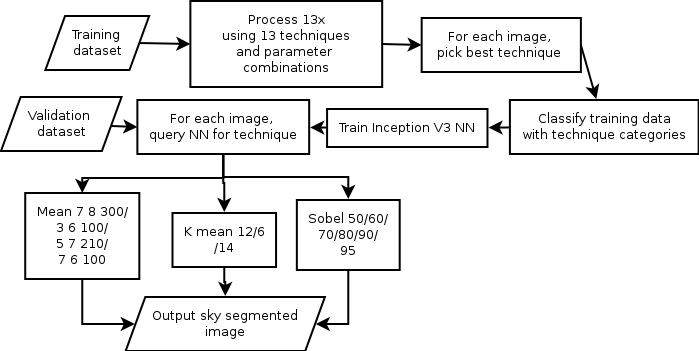
\includegraphics[scale=0.70]{Images/TrainingProcessDiagram}
\caption{\bf Process flow of training and validation steps.}    
 \label{fig:process}  
\end{figure} 


\subsection{Data overview}\label{sec:data}
Overall, 38,521 images of outdoor scenes were used, 38,115 from the Skyfinder dataset and 406 from GSV. During the training and evaluation, the two datasets were combined then split into 28,886 training and 9635 validation images.


\subsubsection{Skyfinder data}\label{sec:finderdata}
This dataset was built from 90,000 long-term timelapse images from 53 outdoor webcams over a variety of lighting and weather conditions. Images are of a wide range of sizes and aspect ratios, including 640x489, 857x665, 960x600, 1280x720, and 1280x960. For each location, a binary sky mask was created for validation purposes. In this study, we selected 38,115 images from 40 locations. Night-time and images with heavy fog were removed as these are conditions unlikely to be encountered in imagery used to calculate sky view factor (i.e. Google Street View).

\subsubsection{GSV data}\label{sec:gsvdata}
Panoramas for 406 locations in a variety of cities (Adelaide, Brisbane, Paris, Sydney, Tokyo, Perth, and Melbourne) were retrieved using the Google Maps API \citep{GoogleMaps2017b}. Images were retrieved as six 640x640 tiles for up, down, left, right, front, and back directions. The six images were stiched together into a 1280x960 cubic image using Java 8 \citep{Oracle2018} and OpenCV\citep {Bradski2000}. Validation images were created by hand marking sky pixels for each image using the GNU Image Manipulation Program \citep{GIMP2019}.

\subsection{Techniques and parameters}
Fourteen different variations of computer vision techniques and parameters were tested and used in this project. They are detailed in Tables \ref{tab:techniques}, \ref{tab:techniques4}, \ref{tab:techniques2}, and \ref{tab:techniques3} and in the following sections.

\begin{table}[!htbp]
\caption{\bf Techniques used for sky pixel detection.  \label{tab:techniques}}     
\begin{tabular}{ l  l l}
\textbf{Technique designations} & \textbf{Technique}  \\ \hline
Sobel  & Sobel operator/hybrid probability model \\	
Mean &  Mean shift \\
K-means  & K-means clustering and HSL color filtering \\
Sobel/flood-fill  & Sobel operator/flood-fill \\
\hline
\end{tabular}
\end{table}

\begin{table}[!htbp]
\caption{\bf Sobel hybrid probability model designations and parameters used for each  \label{tab:techniques4}}     
\begin{tabular}{ l  l }
\textbf{Designation}  & \textbf{Threshold}    \\ \hline
Sobel\_50 & 0.5 \\	  
Sobel\_60 & 0.6 \\	
Sobel\_70 & 0.7 \\	
Sobel\_80 & 0.8 \\
Sobel\_90 & 0.9 \\
Sobel\_95 & 0.95 \\
\hline
\end{tabular}
\end{table}

\begin{table}[!htbp]
\caption{\bf Mean shift designations and parameters used for each \label{tab:techniques2}}     
\begin{tabular}{ l  l  l l}
\textbf{Designation}  & \textbf{Spatial radius (pixels)}&\textbf{Range radius (pixels)}&\textbf{Min. density (pixels)}   \\ \hline
Mean\_7\_8\_300 & 7 & 8& 300 \\
Mean\_3\_6\_100	 & 3& 6& 100 \\
Mean\_5\_7\_210	 & 5& 7& 210 \\	 
Mean\_7\_6\_100	 & 7& 6& 100 \\

\hline
\end{tabular}
\end{table}

\begin{table}[!htbp]
\caption{\bf K-means designations and parameters used for each \label{tab:techniques3}}     
\begin{tabular}{ l l l l l l l l}
\textbf{Designation} & \textbf{Clusters} & \textbf{Skyreq}&\textbf{H$_{uplimit}$}&\textbf{H$_{downlimit}$} & \textbf{L$_{lightness}$} & \textbf{L$_{gray}$}& \textbf{S$_{gray}$} \\ \hline
K-mean\_12  & 12 & 0.7& 0.75& 0.3 & 0.95 & 0.75 & 0.2 \\
K-mean\_6  & 6 & 0.6& 0.75& 0.3 & 0.95 & 0.75 & 0.2 \\
K-mean\_14  & 14 & 0.4& 0.75& 0.3 & 0.95 & 0.65 & 0.2 \\
\hline
\end{tabular}
\end{table}

	


\subsubsection{Hybrid probability model}\label{sec:prob}
An implementation of the sky detection algorithm presented in \cite{Wang2015a} was implemented using OpenCV \citep{Bradski2000} and Java 8 \citep{Oracle2018}. This method proceeds by calculating gray scale gradient images using x- and y-directional Sobel operators to estimate sky color. An object function attempts to find the best sky-ground boundary in the gradient image using the covariance matrices of a first calculation of sky and ground regions. Using this best sky boundary, the image is again separated into sky and ground regions and a probability model is created from the center and standard deviations of the colors. A second probability model is created from the gradient values. A third probability model is built based on the vertical position of each pixel (vertically higher pixels are more likely to be sky). An overall probability model, ranking each pixel's probability (0 to 1) to be sky, is generated by applying close operations on the three probability models. \cite{Wang2015a} did not recommend a probability threshold, so a number of thresholds were tested (0.5, 0.6, 0.7, 0.8, 0.9, and 0.95). The technique designations and thresholds are detailed in Table \ref{tab:techniques4}. The algorithm was applied to each image and pixels that exceeded the chosen threshold were marked as sky pixels (using blue, RGB 0,0,255). \cite{Wang2015a} reports an error average (in percent of sky) of 0.051 and standard deviation of 0.058 in their evaluation using human-labeled images.  Example results from our implementation are shown in Figure \ref{fig:sobolresults}. 



\begin{figure}
\centering    
a)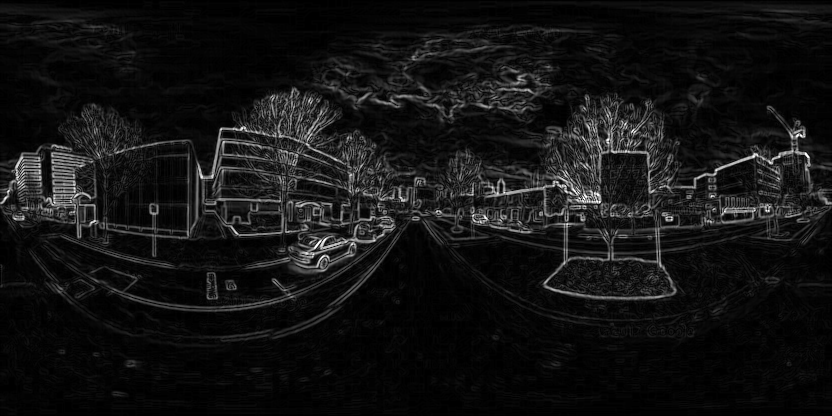
\includegraphics[scale=0.20]{Images/panorama-ESuX4xmQ_fDc50NK6CnfZQ-1_Sobel.png} 
b)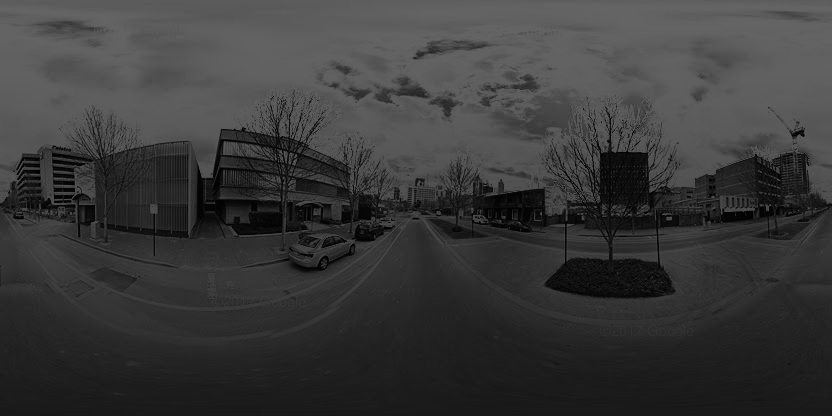
\includegraphics[scale=0.20]{Images/panorama-ESuX4xmQ_fDc50NK6CnfZQ-1_Sobel_prob.png} 
c)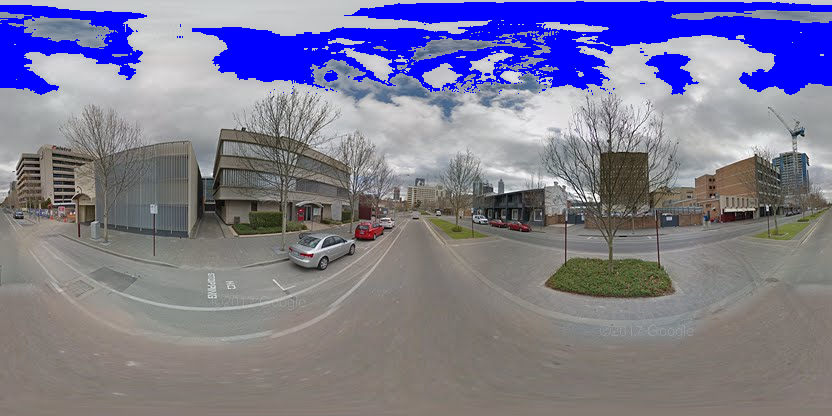
\includegraphics[scale=0.20]{Images/panorama-ESuX4xmQ_fDc50NK6CnfZQ-1_Sobel_95_marked.png} 
d)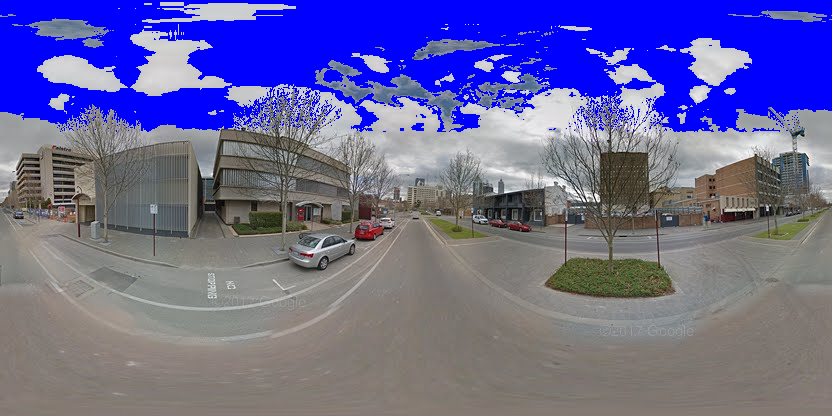
\includegraphics[scale=0.20]{Images/panorama-ESuX4xmQ_fDc50NK6CnfZQ-1_Sobel_90_marked.png} 
e)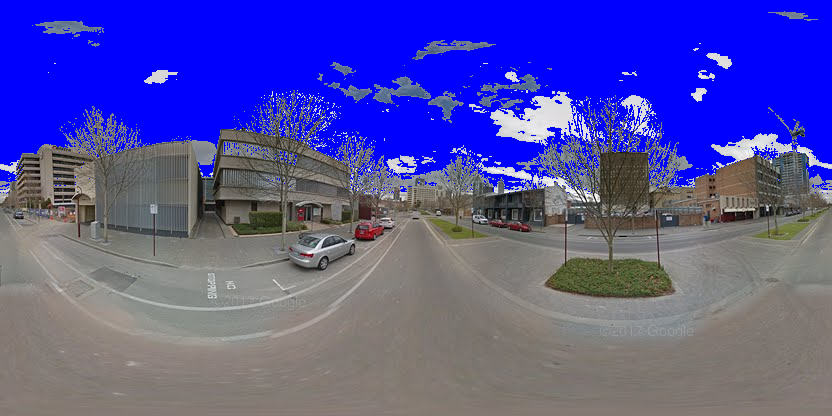
\includegraphics[scale=0.20]{Images/panorama-ESuX4xmQ_fDc50NK6CnfZQ-1_Sobel_80_marked.png} 
f)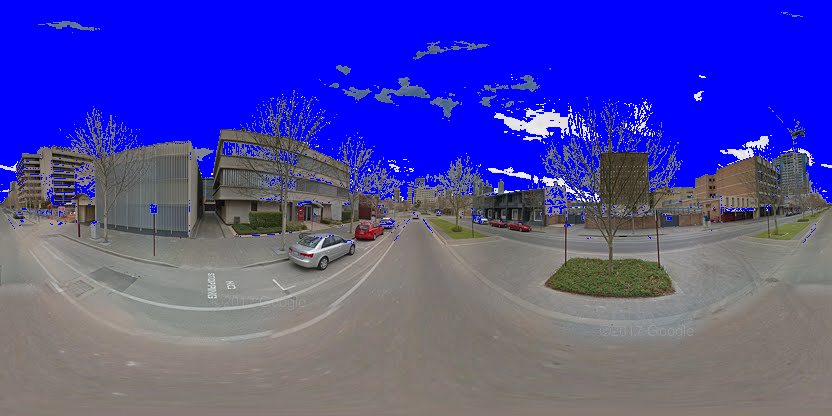
\includegraphics[scale=0.20]{Images/panorama-ESuX4xmQ_fDc50NK6CnfZQ-1_Sobel_70_marked.png} 
g)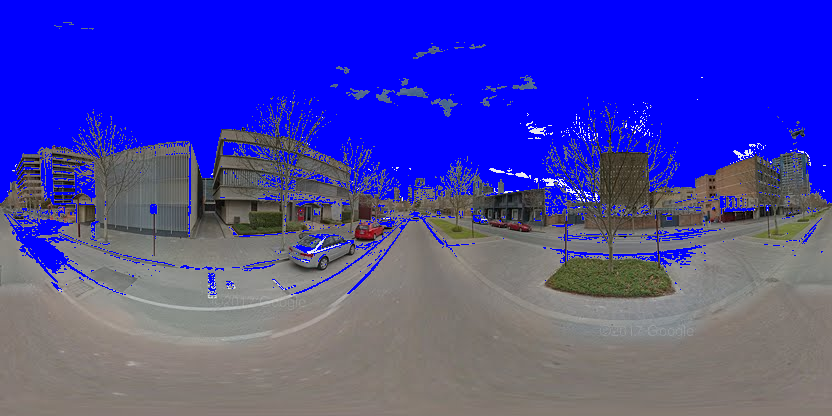
\includegraphics[scale=0.20]{Images/panorama-ESuX4xmQ_fDc50NK6CnfZQ-1_Sobel_60_marked.png} 
h)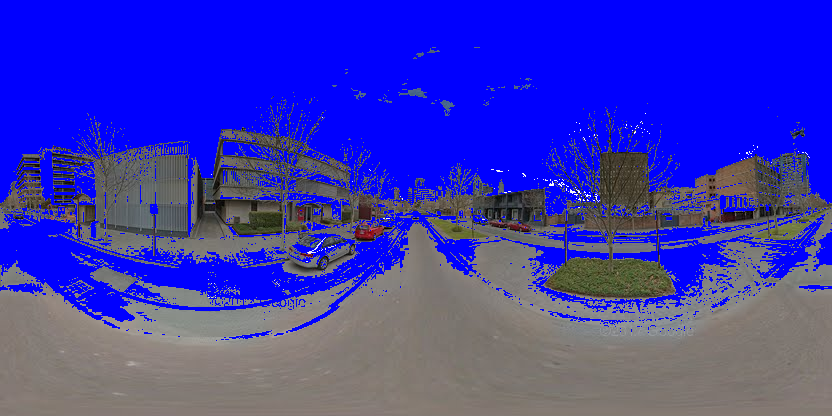
\includegraphics[scale=0.20]{Images/panorama-ESuX4xmQ_fDc50NK6CnfZQ-1_Sobel_50_marked.png} 
\caption{\bf  Results of hybrid probability model, showing a) Sobel operator gradient image, b) resulting probability predictions, c) Sobel\_50, d) Sobel\_60, e) Sobel\_70, f) Sobel\_80, g) Sobel\_90, and h) Sobel\_95.}    
 \label{fig:sobolresults}  
\end{figure} 

\subsubsection{Mean shift}\label{sec:mean}

Mean shift is an algorithm often used for image segmentation \citep{Comaniciu1997,Comaniciu2002}. Image segmentation involves decomposing images into homogeneous contiguous regions of pixels of similar colours or grey levels. Mean shift uses an iterative algorithm to pick search windows of a certain radius ($r$) in an initial location in an image, then compute a mean shift vector and translate the search window by that amount until convergence \citep{Comaniciu1997}. Segmentation results are highly dependent on input parameters for the algorithm, which include the spatial radius of the search window, colour range radius of the search window, and minimum density (the minimum number of pixels to constitute a region). The mean shift used in this project is based on a Java port by \cite{Pangburn2002} of the C++ based EDISON vision toolkit \citep{Christoudias2002}. Four different variations of the input parameters were used, determined experimentally through a sensitivity test to work across the widest variety of images. The technique designations and parameters are detailed in Table \ref{tab:techniques2}. Mean shift is applied to each image with the chosen set of parameters and pixels of the most common colour (in the top half of the image) are marked as sky (using blue, RGB 0,0,255). Example results are shown in Figure \ref{fig:meanresults}.


\begin{figure}
\centering    
a)\includegraphics[scale=0.25]{Images/panorama-ESuX4xmQ_fDc50NK6CnfZQ-1_cropped.png} 
b)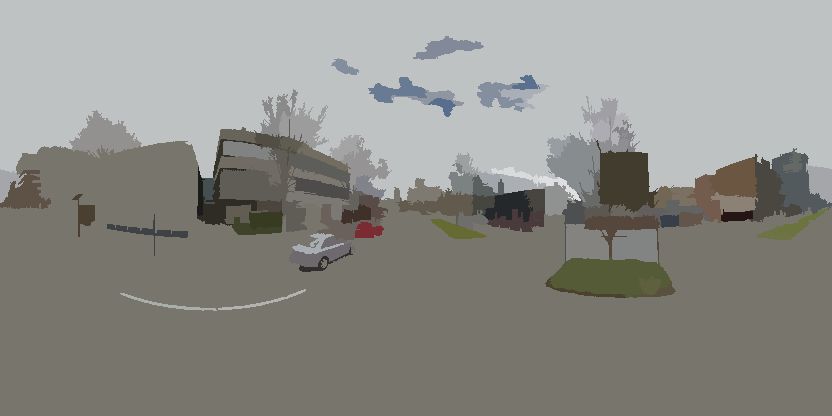
\includegraphics[scale=0.25]{Images/panorama-ESuX4xmQ_fDc50NK6CnfZQ-1_seg.png} 
c)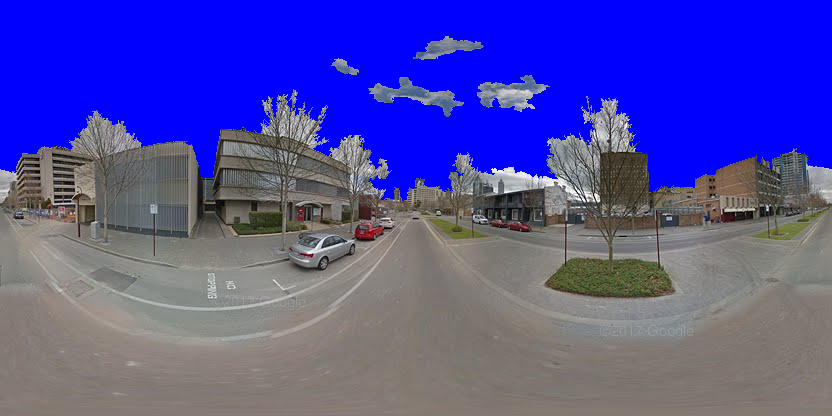
\includegraphics[scale=0.25]{Images/panorama-ESuX4xmQ_fDc50NK6CnfZQ-1_ms_sky_mark.png} 
\caption{\bf Results of mean shift (Mean\_5\_7\_210) showing a) original image, b) mean shifted image, and c) final marked image.}    
 \label{fig:meanresults}  
\end{figure} 



\subsubsection{K-means clustering and HSL color filtering}\label{sec:kmeans}
A third sky segmentation technique was designed using K-means clustering and hue, saturation, and lightness (HSL) colour filtering. K-means clustering iteratively splits an image into $K$ number of clusters, terminating when a specified criteria is met (i.e. maximum iterations and/or desired accuracy). The K-means clustering was performed using the K-means method from the OpenCV library \citep{Bradski2000}. Three different input parameters variations were used, determined experimentally through a sensitivity test to work on a wide variety of images. The technique designations and parameters are detailed in Table \ref{tab:techniques3}. 

K-means clustering was performed on each image, splitting the image into the chosen number of clusters. Filtering cluster regions was based on HSL values. The following conditions (for $H$, hue, $S$, saturation, and $L$, lightness) must be met to add a colour region to a list of possible sky regions: 

$H_{downlimit} < H < H_{uplimit}$

$\cup L > L_{lightness}$

$\cup L > L_{gray} \cap S < S_{gray}$

Of these possible sky clusters, only clusters with a number of pixels greater than the $Skyreq$ threshold (percent of all pixels) in the image were finally marked as sky regions (using blue, RGB 0,0,255). Example results are shown in Figure \ref{fig:kmeansresults}. 


\begin{figure}
\centering    
a)\includegraphics[scale=0.20]{Images/Cloudy/panorama-ESuX4xmQ_fDc50NK6CnfZQ-1_cropped.png} 
b)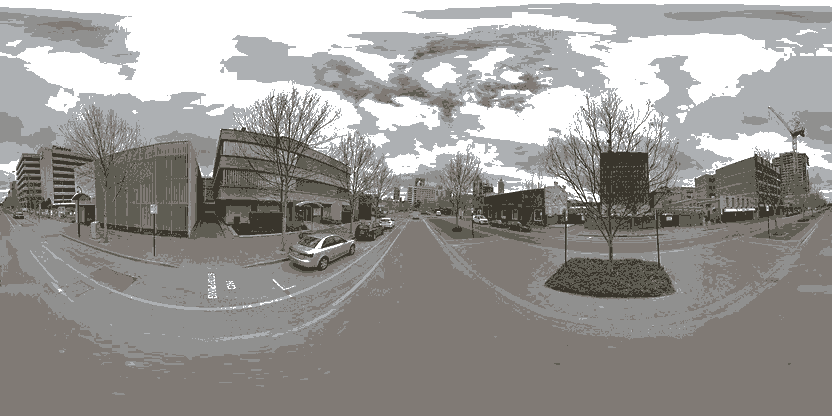
\includegraphics[scale=0.20]{Images/Cloudy/panorama-ESuX4xmQ_fDc50NK6CnfZQ-1_clustered6.png} 
c)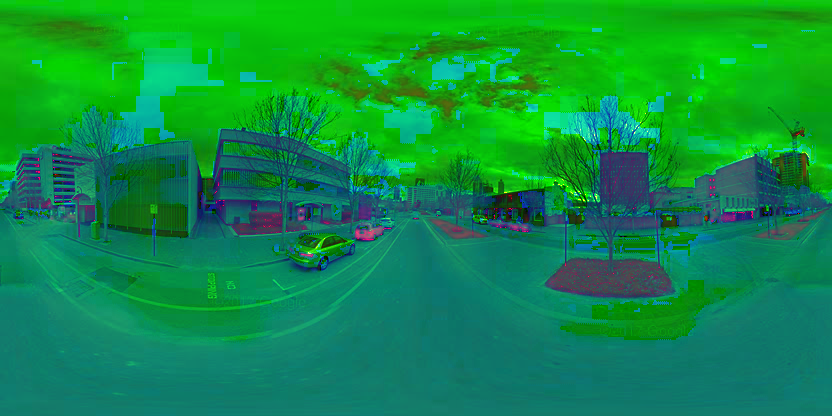
\includegraphics[scale=0.205]{Images/Cloudy/panorama-ESuX4xmQ_fDc50NK6CnfZQ-1_HLS6.png} 
d)\includegraphics[scale=0.20]{Images/Cloudy/{panorama-ESuX4xmQ_fDc50NK6CnfZQ-1_sky_mark0.4}.png} 
\caption{\bf  Results of K-means clustering (K-mean\_6) and HSL filtering, showing a) original image, b) K-means clustered image, c) HSL intermediate image, and d) final marked image.}    
 \label{fig:kmeansresults}  
\end{figure} 



\subsubsection{Sobel operator and flood-fill combination}\label{sec:floodfill}

\cite{Middel2018} developed a process based on a Sobel filter and flood-fill algorithm \citep{Sobel1968,Laungrungthip2008,Middel2017}. This method was designed to calculate sky view factor from Google Street View panorama images that had the bottom half cropped off and were converted to a fisheye projection. \cite{Middel2018}'s evaluation against 1.6 million locations deep learning classified images reported error rates of RMSE (in SVF) of 0.045 and a R$^{2}$ of 0.880. All 38,521 images in the combined training and validation dataset were processed with this algorithm (sky pixels marked with white, RGB 255,255,255), compared to validation images, and results saved for a comparison with our process flow results.  Example results are shown in Figure \ref{fig:sobelflood}. 



\begin{figure}
\centering    
\fbox{
a)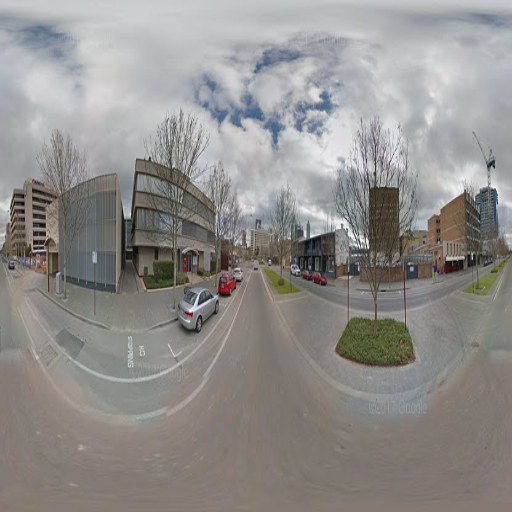
\includegraphics[scale=0.20]{Images/FloodfillInput.png}
b)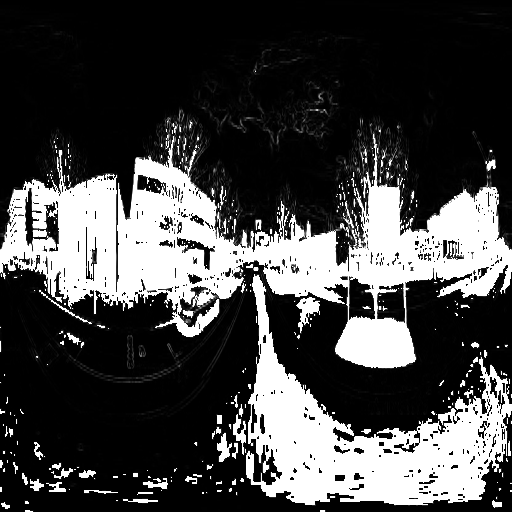
\includegraphics[scale=0.20]{Images/FloodfillMiddle.png}
c)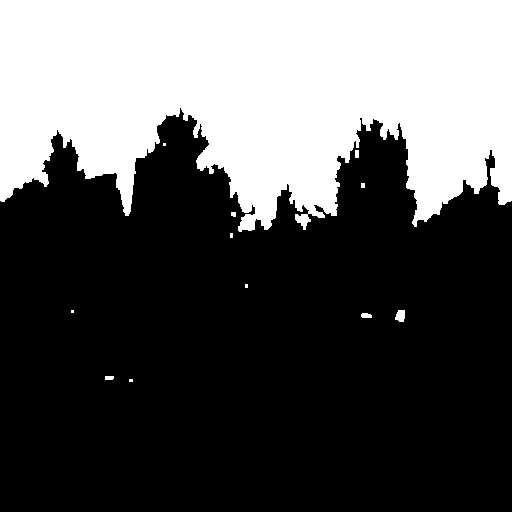
\includegraphics[scale=0.20]{Images/FloodfillOutput.png}
}
\caption{\bf   Results of Sobel/flood-fill combination, showing a) original image, b) intermediate Sobel image, and c) final marked sky image.}    
 \label{fig:sobelflood}  
\end{figure} 

\subsection{Neural network}\label{sec:nn}

\subsubsection{Inception V3}\label{sec:inception}
The Microsoft Cognitive Toolkit (CNTK) \citep{Yu2015,Agarwal2016}, with the the Inception V3 network \citep{Szegedy2015a}, was used in this project to route images through our adaptive algorithm. This artificial neural network (NN) is a widely used model for image classification across a large variety of fields \citep{Xia2017,Hassannejad2016}. This model is trained by presenting the model with list of images assigned to categories (in our case of which technique performed most accurately for each image) and running the training process until the model reached peak accuracy (convergence).


\subsubsection{Neural network training}\label{sec:nntraining}    

The entire dataset of 38522 images was split into two datasets of 75\% training and 25\% validation. All training and validation images (which consisted of images of a wide variety of sizes and ratios) were rescaled to 300x300. The network was calibrated using supervised learning with the generated dataset to identify one of the 13 sky detection techniques and parameters that performed with the highest accuracy for each image. The neural network was trained for 250 epochs on a Nvidia GeForce GTX 1080 GPU, requiring about 12 hours. The neural network reached peak accuracy (errs=53.445\%; top5Errs=10.782\%) at epoch 182. To avoid overfitting and overtraining, epoch 182 was used for classification. Examples imagery used in training for selected classifications are shown in Figure \ref{fig:classImages}.

%results_per_epoch1:Finished Epoch[182 of 250]: [Validate] ce = 4.20379336 * 9636; errs = 53.445% * 9636; top5Errs = 10.782% * 9636



\begin{figure}
\centering
a)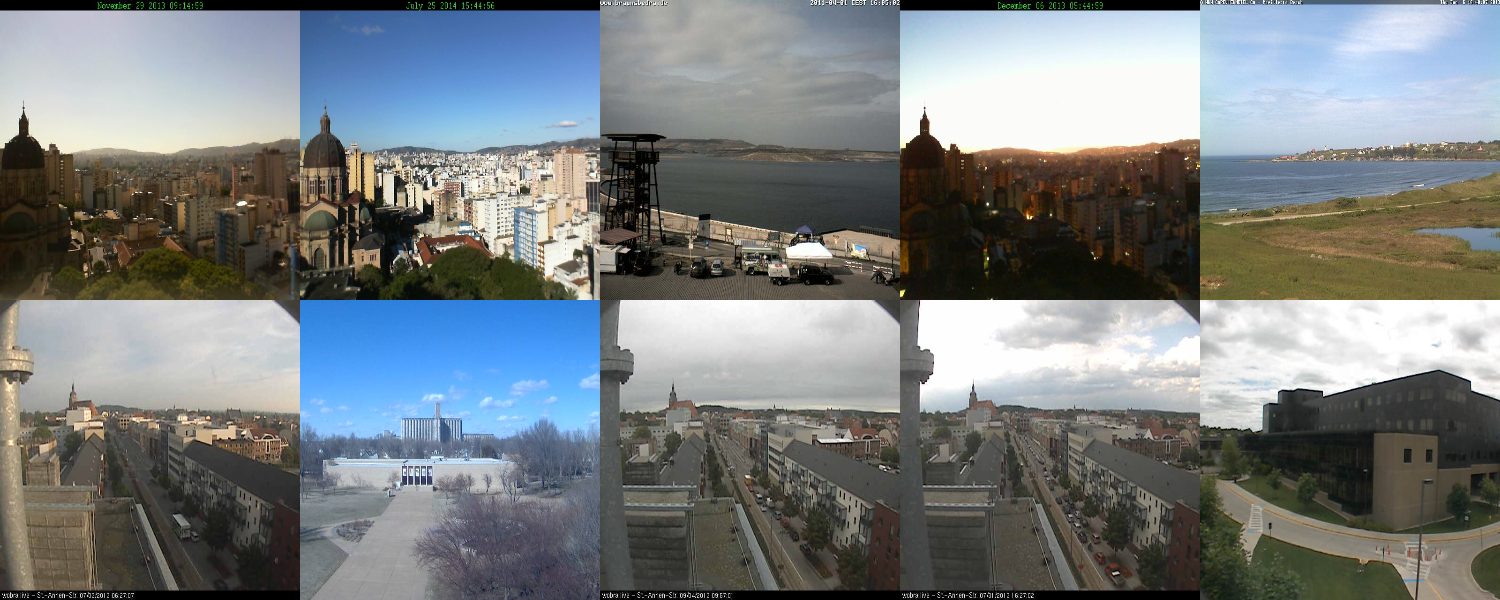
\includegraphics[trim = 0mm 0mm 0mm 0mm,clip,scale=0.12]{Images/13-0_Mean_7_8_300_tiles.png}
b)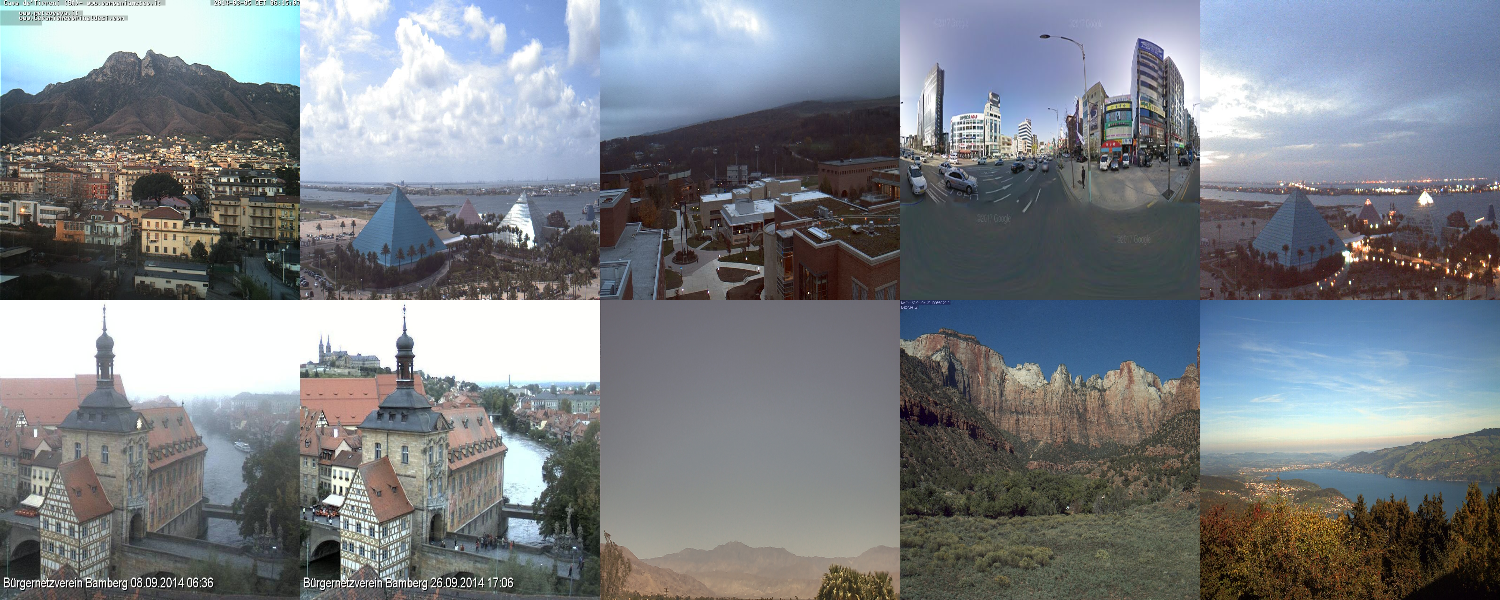
\includegraphics[trim = 0mm 0mm 0mm 0mm,clip,scale=0.12]{Images/13-3_Mean_7_6_100_tiles.png}
c)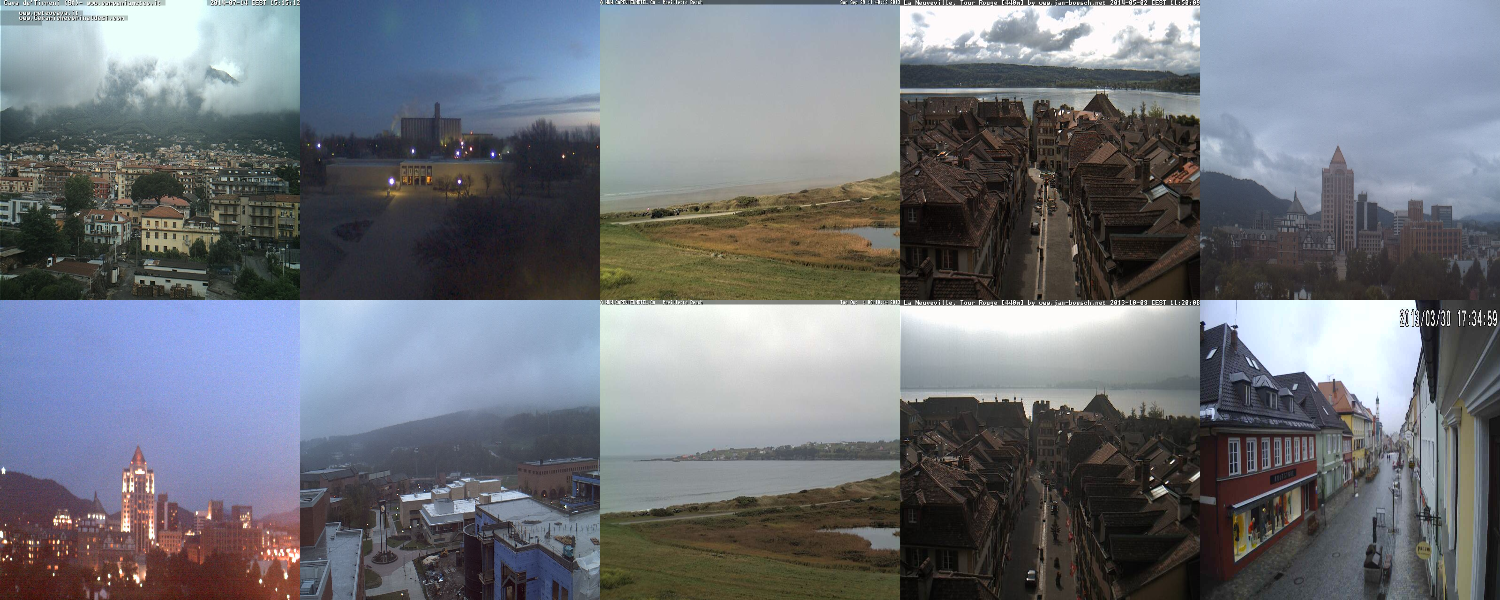
\includegraphics[trim = 0mm 0mm 0mm 0mm,clip,scale=0.12]{Images/13-5_K-mean_6_tiles.png}
d)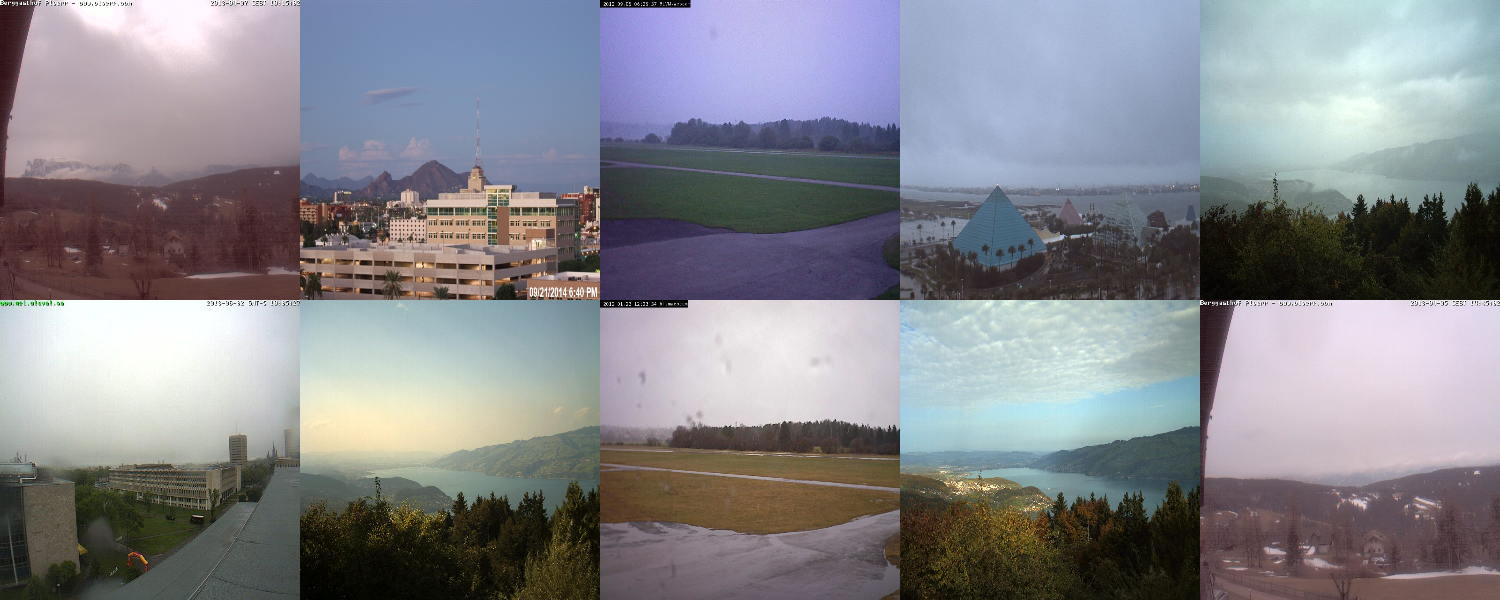
\includegraphics[trim = 0mm 0mm 0mm 0mm,clip,scale=0.12]{Images/13-9_Sobel_70_tiles.png}
\caption{\textbf{Selected imagery used for NN training for classifications 
a) Mean\_7\_8\_300, b) Mean\_7\_6\_100, c) K-mean\_6, d) Sobel\_70.}}
\label{fig:classImages}
\end{figure}



\subsubsection{Neural network inference}\label{sec:nninference}    
Using the trained model from epoch 182, inferences were performed using the 9635 images from the evaluation dataset. Based on the classification picked by the model as being the most probable, the appropriate technique and parameters from that classification was used to mark the sky pixels. The marked image was compared to the validation image and accuracy calculated for each image.

\section{Results}\label{sec:results}

%Overall, 38,521 images were used, 38,115 from the Skyfinder dataset and 406 from Google Street View. During the training and evaluation, the two datasets were combined then split into 28,886 training and 9635 validation images.

There are three sets of results reported in this section. The first is a comparison of all of the techniques and parameters run against the entire combined dataset of 38,521 images. The second presents the results of 9635  validation images using our process flow with the techniques and parameters chosen by the trained NN. The third presents an evaluation of the Sobel/flood-fill algorithm compared to our NN chosen pathway process flow.

\subsection{Results from all techniques}\label{sec:resultsall}
All 14 techniques and parameter combinations were used to process the two datasets of 38,115 Skyfinder, 407 GSV images, and 38,521 combined. A summary of R$^{2}$ and RMSE statistics for evaluations against the three datasets is presented in Table \ref{tab:evalall}. Plots of a number of the better performing techniques are presented in Figure \ref{fig:errorallcombined}. Note, the strong horizontal lines in these figures are due to the nature of the dataset which contains large groups of the same scenes (with the same percentage of sky) under different lighting and weather conditions.

\begin{table}[!htbp]
\caption{\bf Evaluation of all techniques and parameters for Skyfinder dataset, GSV dataset, and combined dataset. (RMSE units in \%/100.) \label{tab:evalall}}     
\begin{tabular}{ l  l l l l l l}
\textbf{Designation}  & \textbf{Skyfinder R$^{2}$} & \textbf{Skyfinder RMSE} & \textbf{GSV R$^{2}$} & \textbf{GSV RMSE} & \textbf{All R$^{2}$} & \textbf{All RMSE} \\ \hline
Mean\_7\_6\_100	&0.746&0.104&0.484&0.076&0.749&0.104 \\
Sobel\_70 &0.395&0.134&0.056&0.107&0.398&0.133 \\
Mean\_5\_7\_210	&0.658&0.142&0.489&0.073&0.661&0.141 \\
Mean\_7\_8\_300 &0.645&0.143&0.505&0.07&0.648&0.142 \\
Mean\_3\_6\_100	&0.657&0.148&0.561&0.066&0.66&0.147 \\
Sobel\_60 &0.288&0.104&0.003&0.188&0.288&0.165 \\
Sobel\_80 &0.254&0.177&0.436&0.07&0.259&0.176 \\
Sobel/flood-fill &0.134&0.211&0.067&0.312&0.13&0.212 \\
Sobel\_50 &0.104&0.23&0.021&0.303&0.103&0.231 \\
Sobel\_90 &0.041&0.317&0.212&0.144&0.04&0.316 \\
K-mean\_6 &0.022&0.325&0.007&0.155&0.022&0.323 \\
K-mean\_14 &0.029&0.328&0.019&0.233&0.029&0.327 \\
K-mean\_12 &0.028&0.343&0.017&0.264&0.03&0.342 \\
Sobel\_95 &0&0.421&0.045&0.225&0.0&0.419 \\
\hline
\end{tabular}
\end{table}



\begin{figure}
\centering
a)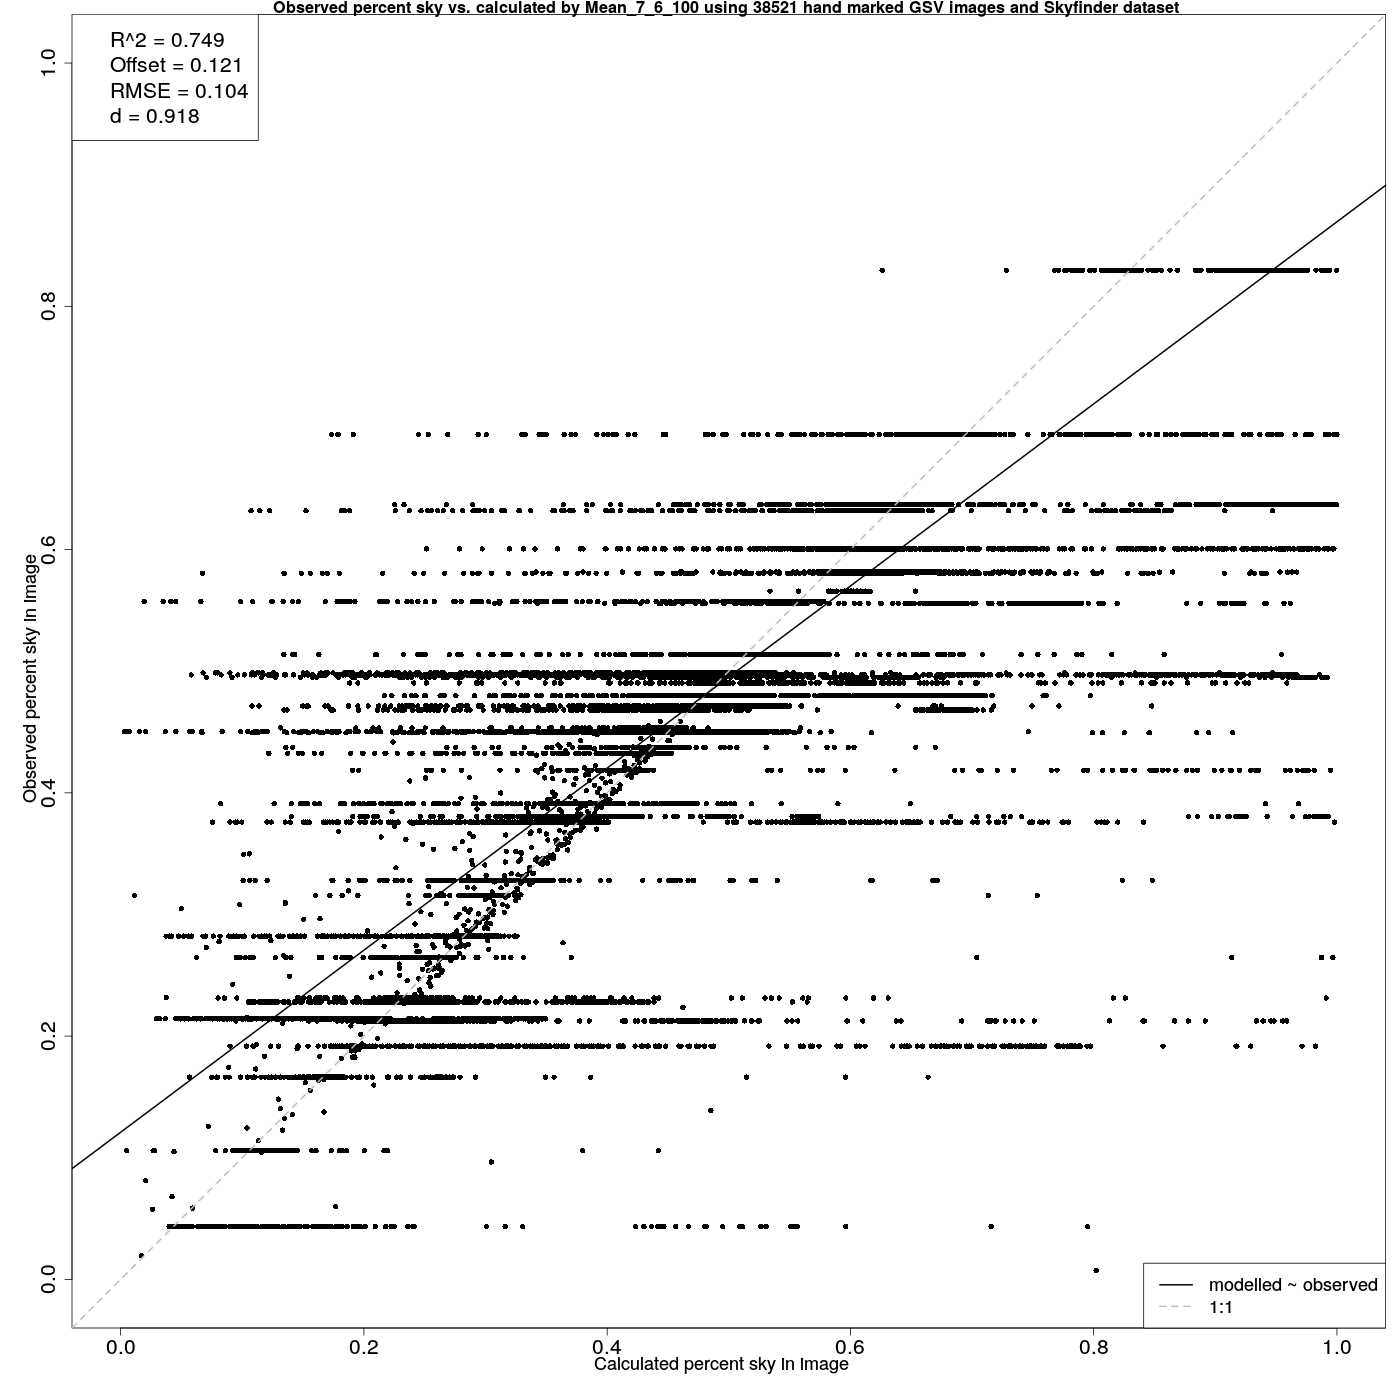
\includegraphics[scale=0.12]{Images/ErrorPlotsCombinedIndivMean_7_6_100.png}
b)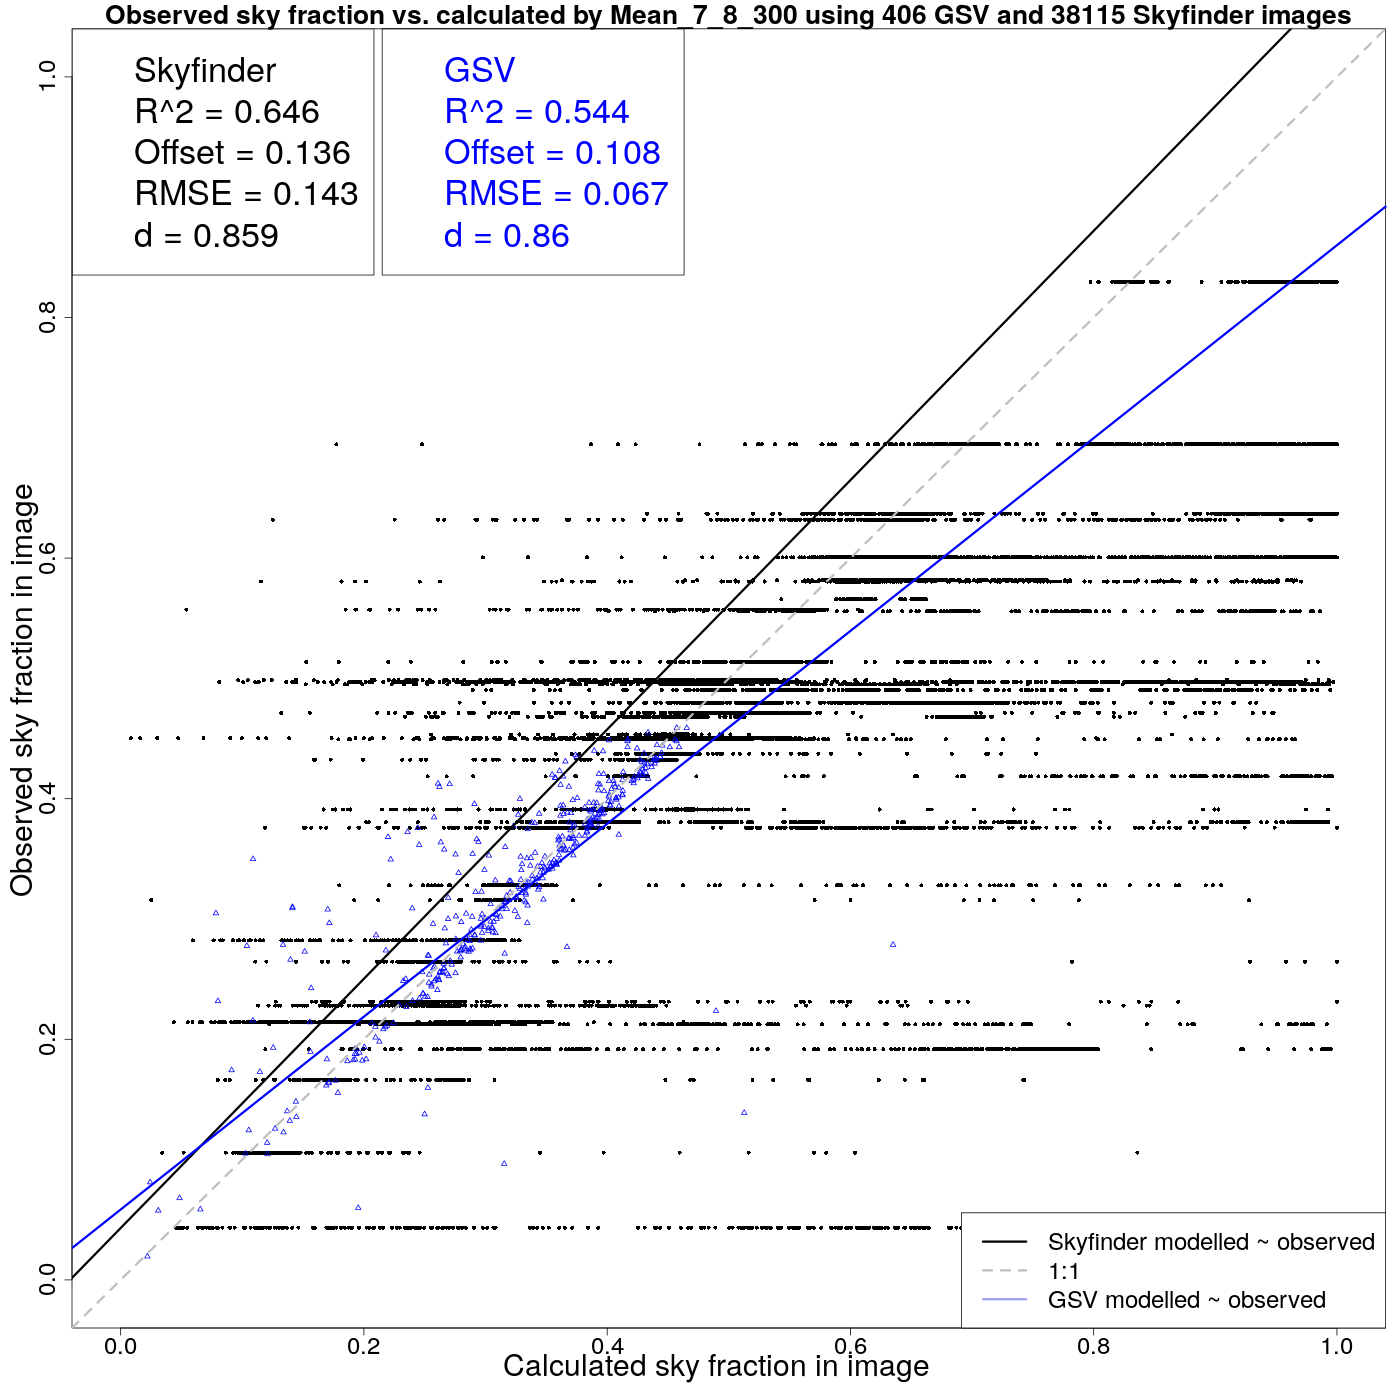
\includegraphics[scale=0.12]{Images/ErrorPlotsCombinedIndivMean_7_8_300.png}
c)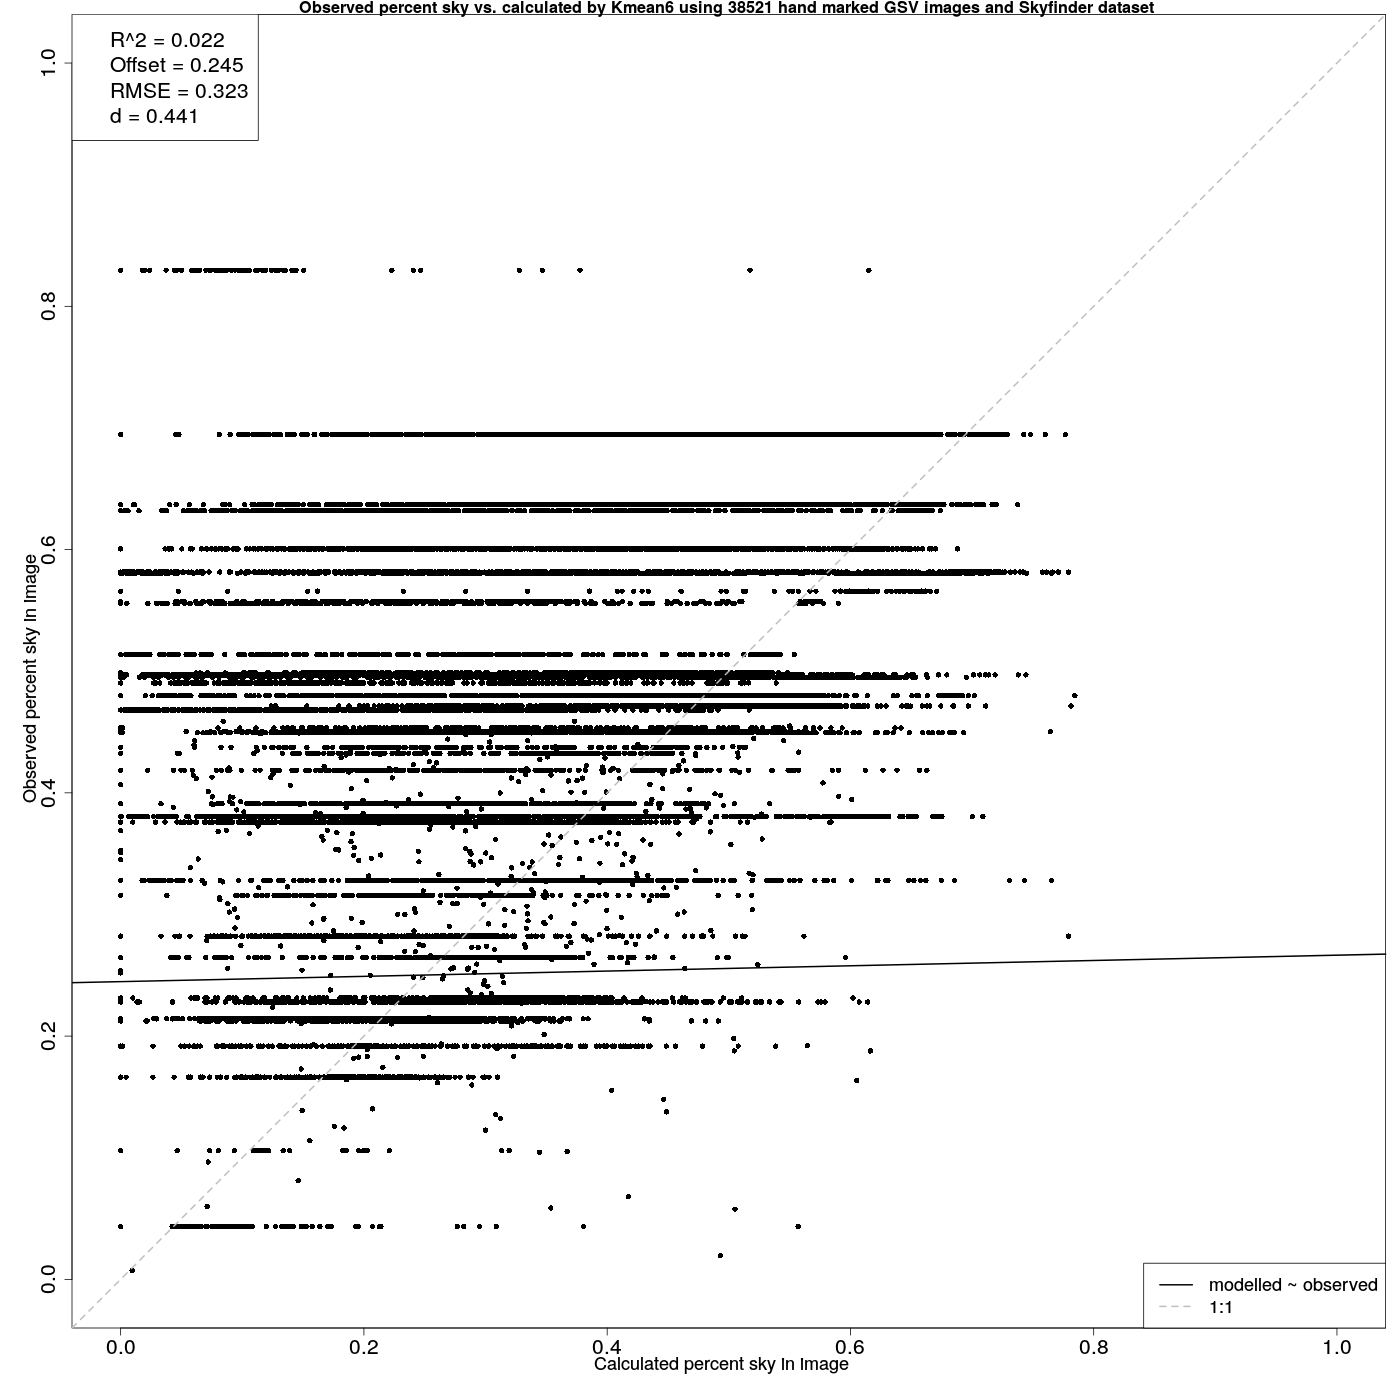
\includegraphics[scale=0.12]{Images/ErrorPlotsCombinedIndivKmean6.png}
d)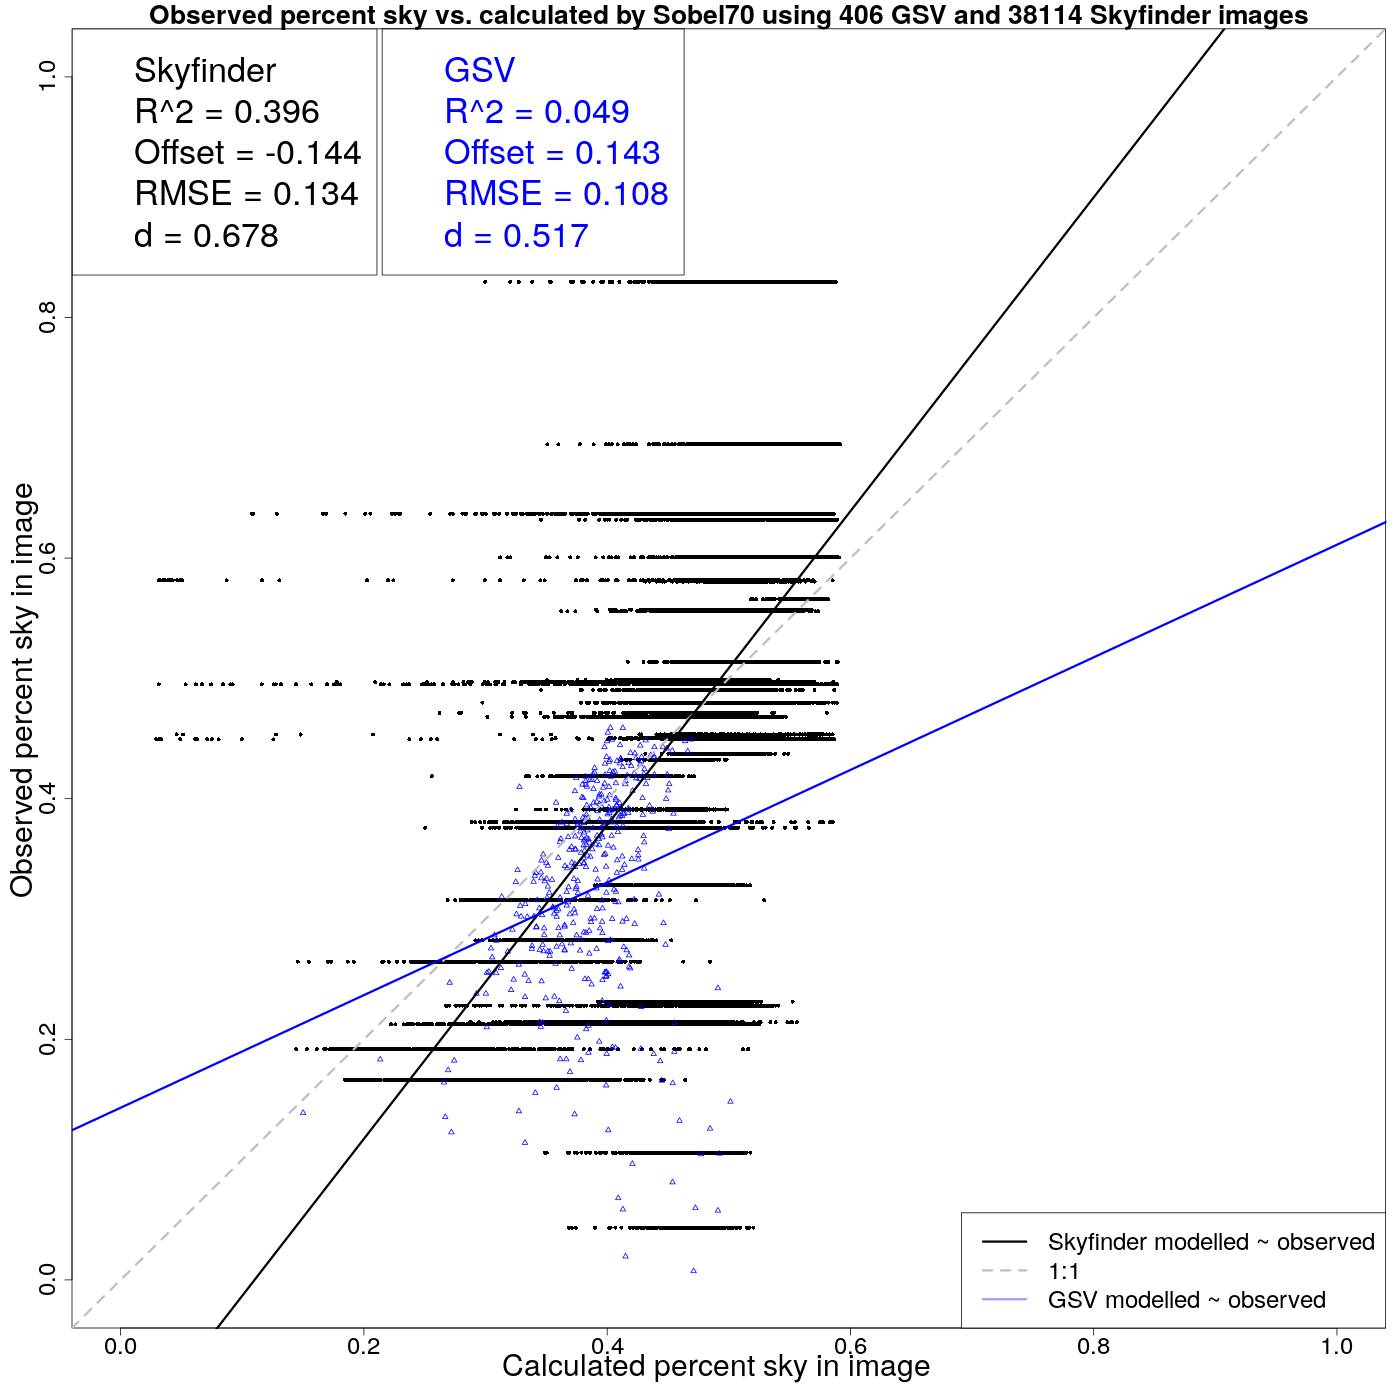
\includegraphics[scale=0.12]{Images/ErrorPlotsCombinedIndivSobel70.png}
\caption{\textbf{Observed vs. calculated sky pixels using the a) Mean\_7\_6\_100, b) Mean\_7\_8\_300, c) K-mean\_6, and d) Sobel\_70 techniques on the 38,521 image combined dataset.} }
\label{fig:errorallcombined}
\end{figure}

\subsection{Results from neural network classified techniques}\label{sec:resultsnn}
Figure \ref{fig:errorplots} presents a theoretical best case. If the NN was 100\% accurate in picking the best technique from the thirteen possible combinations based on its training, a RMSE of 0.026 and 0.02 is possible against the 38,115 Skyfinder images and 407 GSV images respectively. However, the NN only achieved an accuracy of errs=53.445\% and top5Errs=10.782\% for the 13 classifications. Figure \ref{fig:errorplotscntk} shows the overall accuracy of the NN chosen pathway process flow against the 9636 validation images, with a RMSE of 0.065 and R$^{2}$ of 0.873.

\begin{figure}
\centering
a)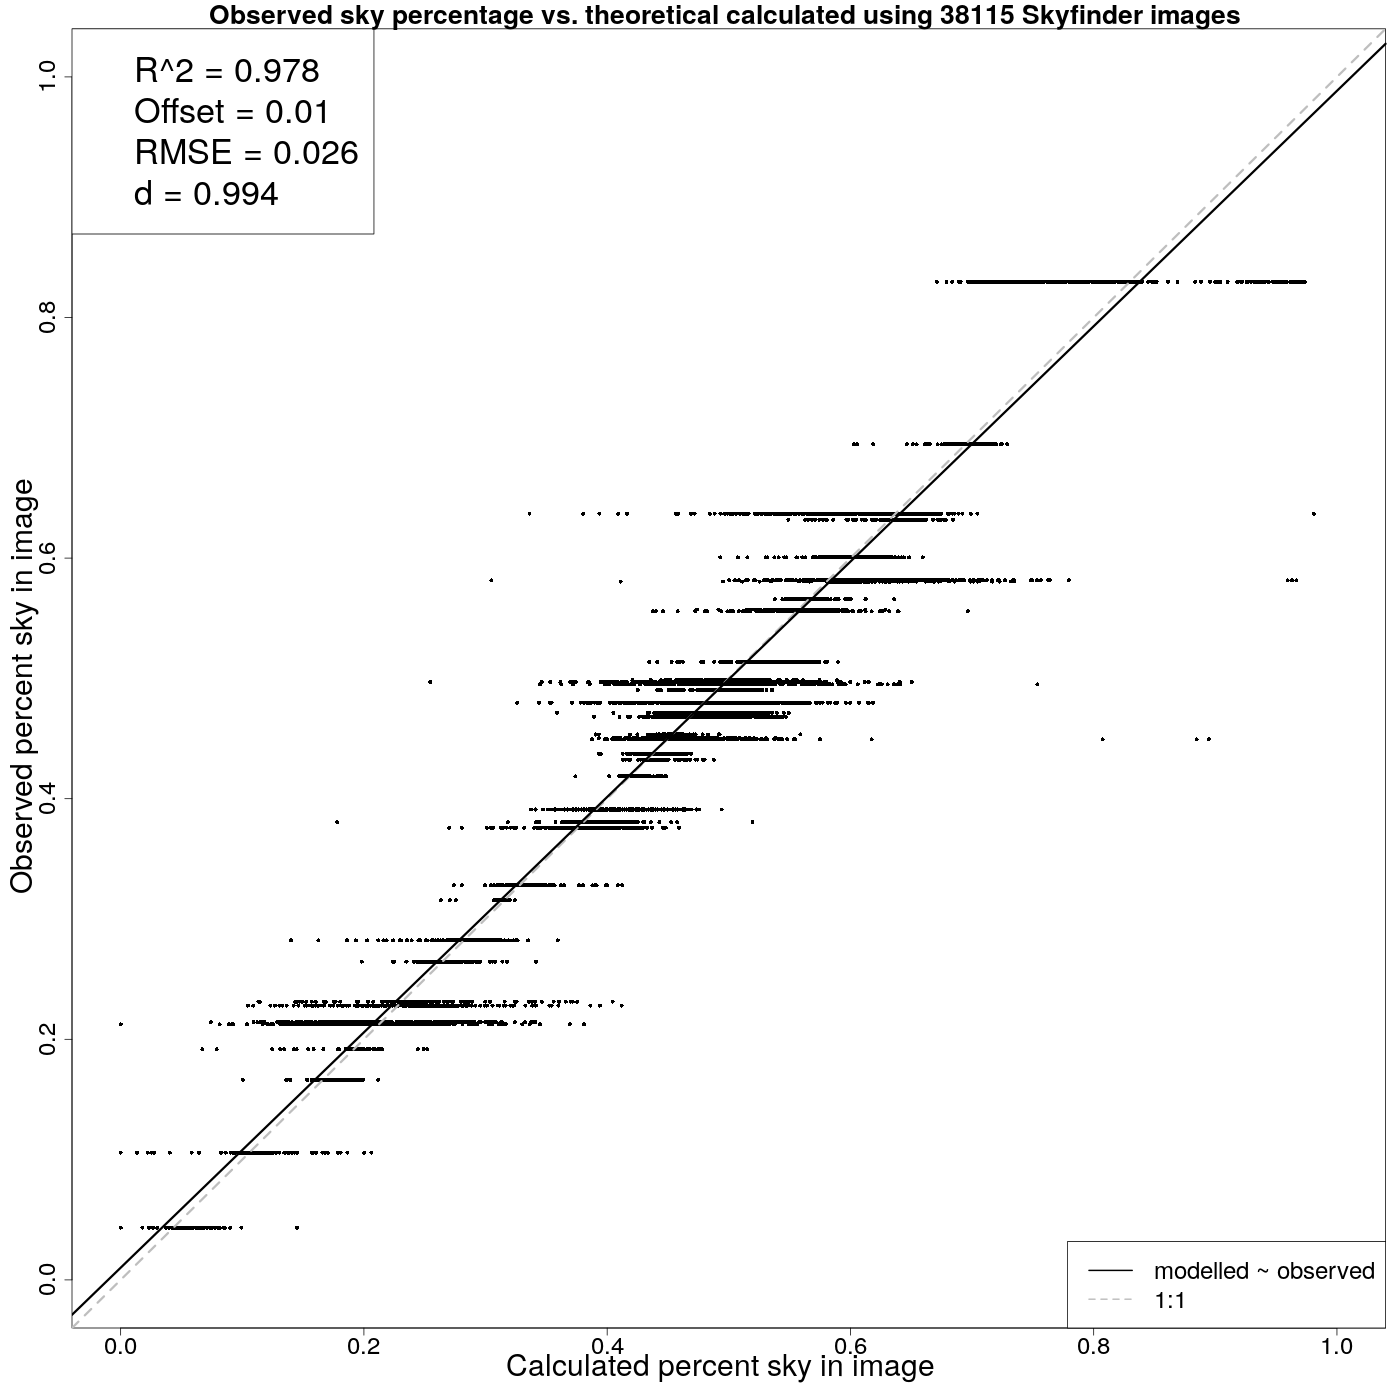
\includegraphics[scale=0.12]{Images/ErrorPlots.png}
b)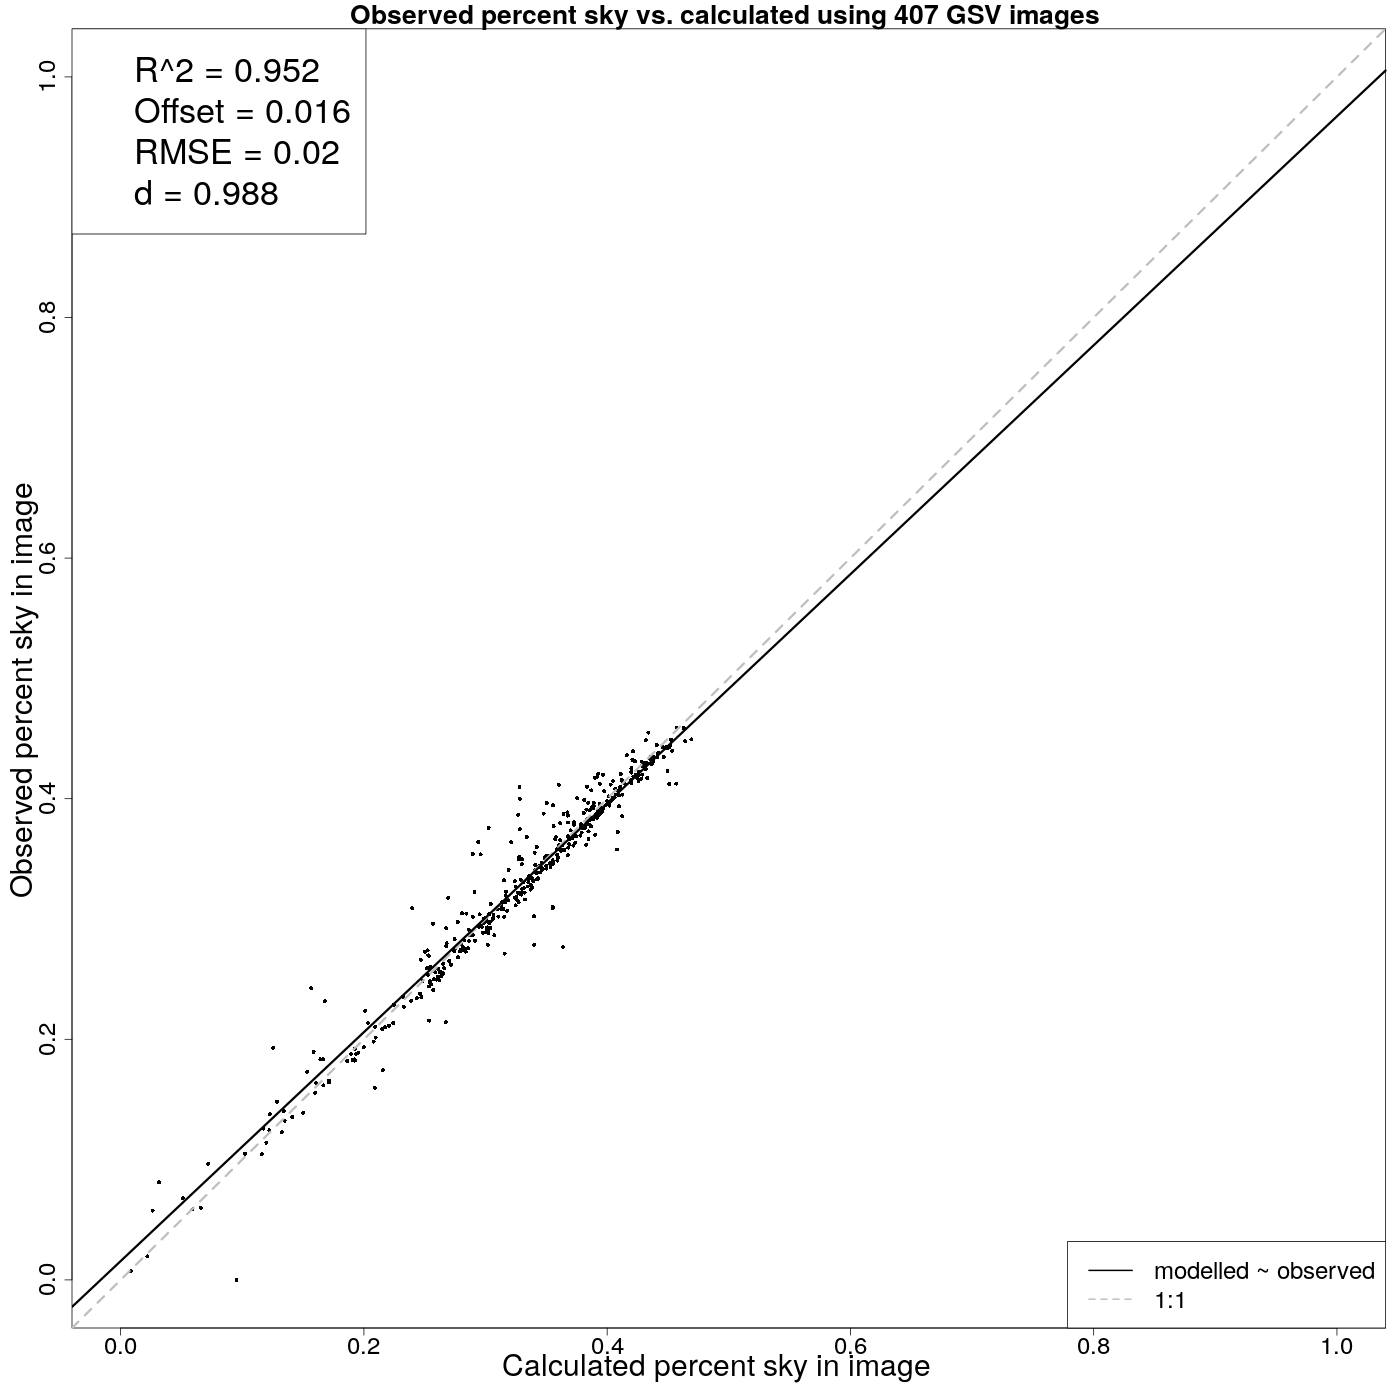
\includegraphics[scale=0.12]{Images/ErrorPlots2.png}
\caption{\textbf{Theoretical best case results if the NN is 100\% accurate for a) Skyfinder and b) GSV datasets.}}
\label{fig:errorplots}
\end{figure}


\begin{figure}
\centering
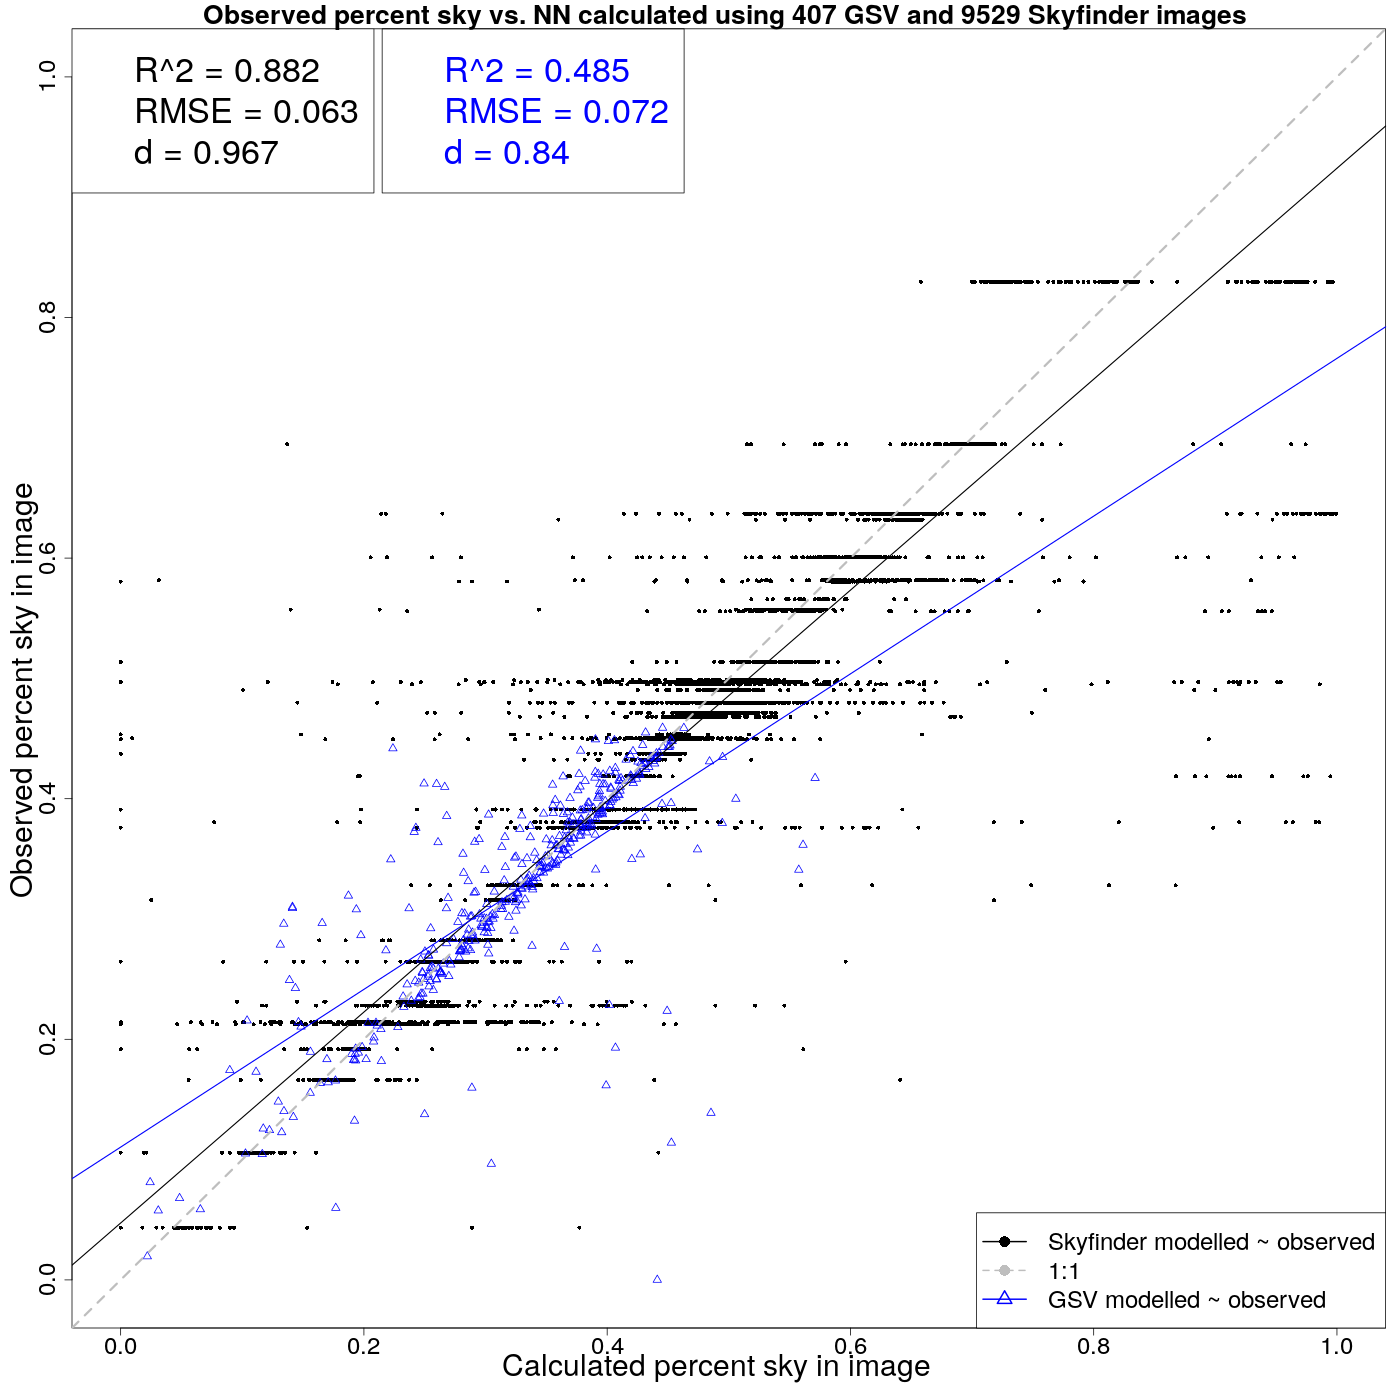
\includegraphics[scale=0.12]{Images/ErrorPlotsCNTK.png}
\caption{\textbf{Results of NN picks against the 9636 validation images.}}
\label{fig:errorplotscntk}
\end{figure}


\subsection{Results from Sobel/flood-fill evaluation}\label{sec:resultsflood}
Finally, in an evaluation of the Sobel/flood-fill algorithm, results against the combined 38,520 image dataset and 9636 validation images are shown in Figure \ref{fig:errorfloodall}. This algorithm shows a RMSE of 0.212 and R$^{2}$ of 0.13 against the combined dataset and a RMSE of 0.205 and R$^{2}$ of 0.15 against the validation dataset.


\begin{figure}
\centering
a)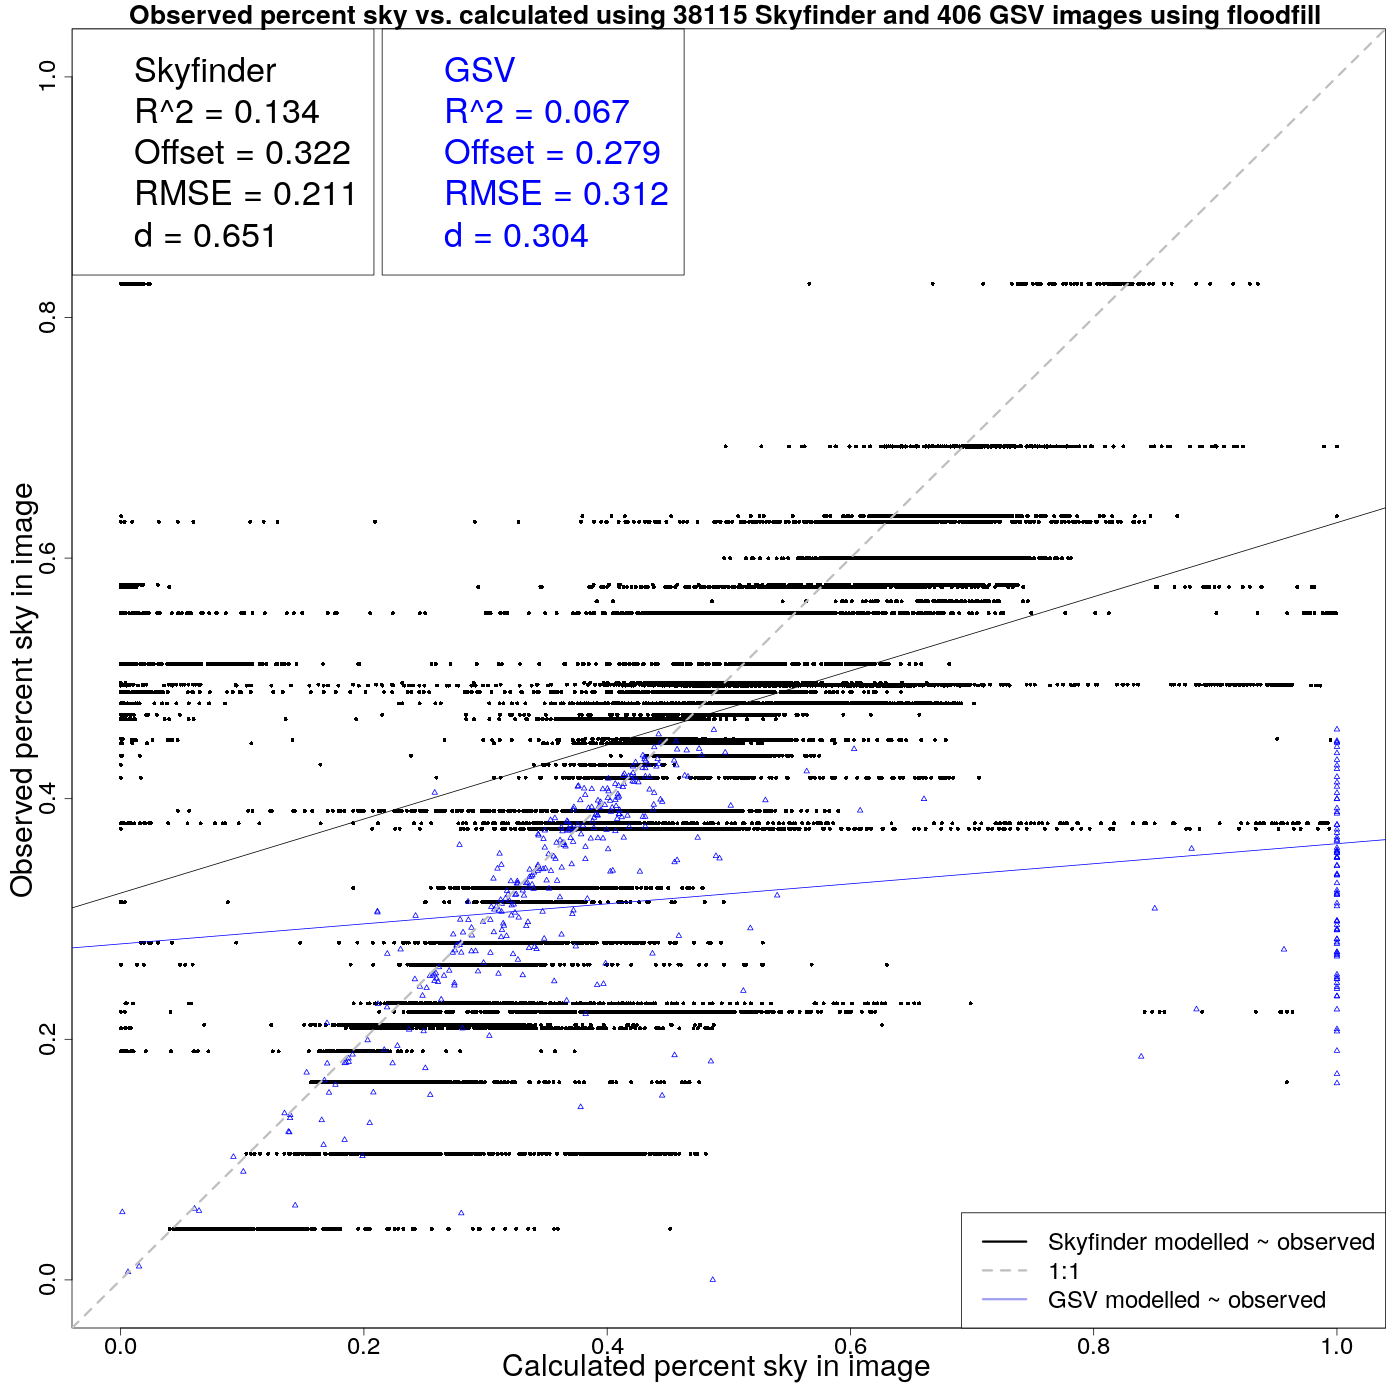
\includegraphics[scale=0.12]{Images/ErrorPlots2FloodfillAll.png}
b)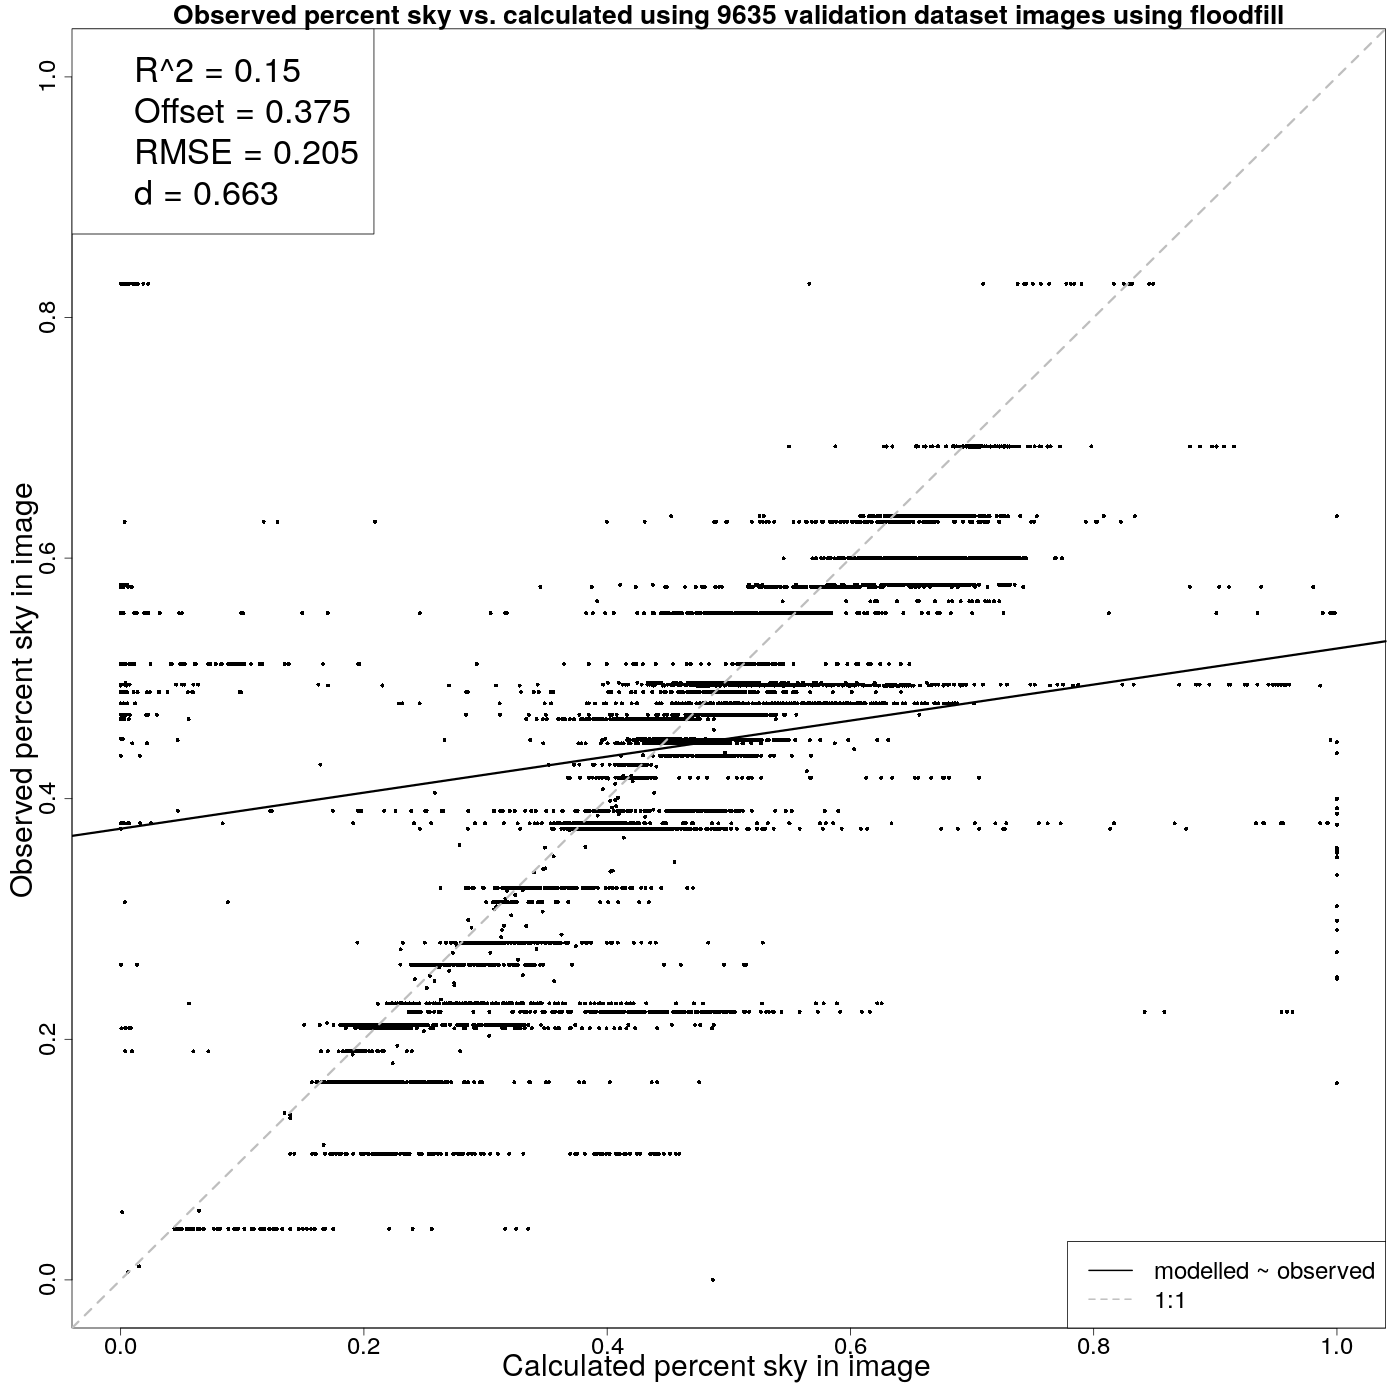
\includegraphics[scale=0.12]{Images/ErrorPlots2FloodfillValidation.png}
\caption{\textbf{Results of Sobel/flood-fill combination against a) combined 38,520 image dataset and b) 9636 validation images.}}
\label{fig:errorfloodall}
\end{figure}


\section{Discussion and conclusion}\label{sec:conclusion}
The results from Section \ref{sec:resultsall} show that no single technique and parameter combination performs sky pixel identification with high accuracy across the dataset used in this project. This dataset contains wide variety of outdoor scenes with a wide range of lighting and weather conditions (as can be seen in some of the sample images in Figure \ref{fig:classImages}). 

At best, all show error rates of 10\% and greater, with some having their overall error rates at 20 and 30\%. However, even the poorest performing techniques showed higher accuracy processing some of the images than all of the other techniques. This validates the need to have an adaptive process that can respond to the specific challenges each image presents to deliver overall better results than any single algorithm is able to.


In addition, having a range of combinations of techniques was important for the overall accuracy. An attempt was made to reduce the number of classifications to possibly increase the accuracy of the NN. While the theoretical accuracy from the 13 classes was a RMSE of 0.026, combinations of the best performing three or four classes saw reduced theoretical accuracy reduced to RMSEs of 0.039 (for Mean\_7\_6\_100, K-mean6, and Sobel\_70), 0.045 (for Mean\_3\_6\_100, K-mean6, and Sobel\_70), 0.036 (for Mean\_7\_6\_100, Mean\_7\_6\_100, K-mean6, and Sobel\_70), or 0.095 (for all Mean combinations). 

The attempt to increase the accuracy of the NN predictions highlights one of the limitations of this study. 53\% error in picking between 13 classes shows that there is much room for improvement. NNs perform best when they are trained with a large amount of data. It this study, there were only 28,885 images in the training dataset. With a larger training dataset resulting in a lower NN error rate, it would be possible to come closer to the theoretical RMSE of 0.026 for the sky pixel identification.

Even with these limitations, in comparison to published methods, the adaptive process performs well. Our accuracy of RMSE of 0.065 compares well to the RMSE of 0.205 for the Sobel/flood-fill and the best performing Sobel (Sobel\_70) which achieved an RMSE of 0.133.


\section{Code and availability and licensing}\label{sec:available}
Code and data are available from the corresponding author on request.

%TARGET is distributed under the Creative Commons Attribution-NonCommercial-ShareAlike 4.0 Generic (CC BY-NC-SA 4.0). TARGET code cannot be used for commercial purposes. It is available in two versions, Python or Java. The Python code can be downloaded from https://doi.org/10.5281/zenodo.1300023 or Java code is available at  https://zenodo.org/record/1310138. We recommend using the Java version as it runs faster than the Python code. 



%\printglossary[title={List of Symbols}]

\section*{Acknowledgements}
The support of the Commonwealth of Australia through the Cooperative Research Centre program is acknowledged. At Monash University, Kerry Nice was funded by the Cooperative Research Centre for Water Sensitive Cities, an Australian Government initiative. At the University of Melbourne, Kerry Nice was funded by the Transport, Health, and Urban Design (THUD) Hub. 
 
%\end{acknowledgements}

\section*{References}\label{sec:ref}
%% If you have bibdatabase file and want bibtex to generate the
%% bibitems, please use
%%
  \bibliographystyle{elsarticle-harv} 
  %\bibliography{library}
  \bibliography{bib}

%% else use the following coding to input the bibitems directly in the
%% TeX file.

%\begin{thebibliography}{00}
%
%%% \bibitem[Author(year)]{label}
%%% Text of bibliographic item
%
%\bibitem[ ()]{}
%
%\end{thebibliography}


%% The Appendices part is started with the command \appendix;
%% appendix sections are then done as normal sections
%\appendix
%\setcounter{table}{0}
%\renewcommand{\thetable}{A\arabic{table}}

%\subsection{}                               %% Appendix A1, A2, etc.


%%%%%%%%%% taking out parameterizations
%\section{Appendix}\label{sec:app}  
%\subsection{Additional data tables}\label{app:tables}  




%\authorcontribution{This work was developed by Kerry Nice and supervised by Andrew Coutts and Nigel Tapper. Model source code was received from Scott Krayenhoff and Remko Duursma (as acknowledged in Section \ref{sec:available}). Synthesis of this code and new code was developed by Kerry Nice. The article was written by Kerry Nice with editing and suggestions from Andrew Coutts and Nigel Tapper.}
%
%\begin{acknowledgements}
%The work described in this paper was developed during a PhD. project at Monash University. Funding for this was obtailed through the City of Melbourne, Monash University, and the CRC for Water Sensitive Cities.  
%\end{acknowledgements}

%\begin{acknowledgements}
%The support of the Commonwealth of Australia through the Cooperative Research Centre program is acknowledged.
%\end{acknowledgements}






\end{document}

\endinput
%%
%% End of file `elsarticle-template-harv.tex'.
